\documentclass[12pt, titlepage]{article}
\usepackage[letterpaper, portrait, margin=1in]{geometry}
\usepackage{booktabs}
\usepackage{tabularx}
\usepackage{hyperref}
\hypersetup{
    colorlinks,
    citecolor=black,
    filecolor=black,
    linkcolor=red,
    urlcolor=blue
}
\usepackage{longtable}
\usepackage[round]{natbib}
\usepackage{colortbl}
\usepackage{graphicx} 
\usepackage{placeins}
\usepackage{array}
\usepackage{float}
\usepackage{colortbl}
\usepackage{caption}
\usepackage{graphicx}
\captionsetup[table]{width=0.9\textwidth}

\usepackage{listings}
\lstset{
    basicstyle=\ttfamily, % Use monospaced font
    breaklines=true,      % Enable line breaks
}
\usepackage{csvsimple}

%% Comments

\usepackage{color}

% \newif\ifcomments\commentstrue %displays comments
\newif\ifcomments\commentsfalse %so that comments do not display

\ifcomments
\newcommand{\authornote}[3]{\textcolor{#1}{[#3 ---#2]}}
\newcommand{\todo}[1]{\textcolor{red}{[TODO: #1]}}
\else
\newcommand{\authornote}[3]{}
\newcommand{\todo}[1]{}
\fi

\newcommand{\wss}[1]{\authornote{blue}{SS}{#1}} 
\newcommand{\plt}[1]{\authornote{magenta}{TPLT}{#1}} %For explanation of the template
\newcommand{\an}[1]{\authornote{cyan}{Author}{#1}}

%% Common Parts

\newcommand{\progname}{Software Engineering} % PUT YOUR PROGRAM NAME HERE
\newcommand{\authname}{\textbf{Team 4, EcoOptimizers} \\
  \\ Nivetha Kuruparan
  \\ Sevhena Walker
  \\ Tanveer Brar
  \\ Mya Hussain
\\ Ayushi Amin} % AUTHOR NAMES

\usepackage{hyperref}
\hypersetup{colorlinks=true, linkcolor=blue, citecolor=blue, filecolor=blue,
urlcolor=blue, unicode=false}
\urlstyle{same}



\begin{document}

\title{Verification and Validation Report: \progname} 
\author{\authname}
\date{\today}
	
\maketitle

\pagenumbering{roman}

\section{Revision History}

\begin{tabularx}{\textwidth}{p{3cm}p{2cm}X}
\toprule {\bf Date} & {\bf Version} & {\bf Notes}\\
\midrule
March 8th, 2025 & 0.0 & Started VnV Report\\
Date 2 & 1.1 & Notes\\
\bottomrule
\end{tabularx}

~\newpage

\section{Symbols, Abbreviations and Acronyms}

\renewcommand{\arraystretch}{1.2}
\begin{tabular}{l l} 
  \toprule		
  \textbf{symbol} & \textbf{description}\\
  \midrule 
  T & Test\\
  \bottomrule
\end{tabular}\\

\wss{symbols, abbreviations or acronyms -- you can reference the SRS tables if needed}

\newpage

\tableofcontents

\listoftables %if appropriate

\listoffigures %if appropriate

\newpage

\pagenumbering{arabic}

This document ...

\section{Functional Requirements Evaluation}
\subsection{Code Input Acceptance Tests}
\begin{enumerate}

\item \textbf{test-FR-1A Valid Python File Acceptance} \\[2mm]
The \textbf{valid Python file acceptance test} ensures that the system correctly processes a syntactically valid Python file without errors. A correctly formatted Python file was provided as input, and the expected result was that the system should accept the file without issue. The \textbf{actual result} confirmed that the system successfully processed the valid file without generating any errors.

\item \textbf{test-FR-1A-2 Feedback for Python File with Bad Syntax} \\[2mm]
This test verifies that the system correctly handles Python files containing deliberate syntax errors. A Python file with syntax errors was fed into the system, and the expected result was that the system should reject the file and provide an appropriate error message indicating the syntax issue. The \textbf{actual result} confirmed that the system correctly identified the syntax errors and displayed the expected error message.

\item \textbf{test-FR-1A-3 Feedback for Non-Python File} \\[2mm]
The \textbf{non-Python file test} ensures that the system correctly rejects unsupported file types and provides clear feedback. A document file (\texttt{document.txt}) and a script with an incorrect file extension (\texttt{script.js}) were tested. The expected result was that the system should reject the files and return an error message indicating that the file format is not supported. The \textbf{actual result} confirmed that the system correctly flagged the non-Python files and provided the appropriate error message.

\end{enumerate}

\subsection{Code Smell Detection and Refactoring Suggestion (RS) Tests}
\begin{enumerate}
    \item \textbf{test-FR-2 Code Smell Detection and Refactoring Suggestion} \\[2mm]
    The \textbf{code smell detection and refactoring tests} validate the system’s ability to identify and refactor specific code smells that impact energy efficiency. These tests ensure compliance with \textbf{functional requirement FR2} and were conducted through unit testing.

    The tester provided Python files containing common code smells such as \textbf{long parameter lists, repeated function calls, and inefficient string concatenation}. The \textbf{expected result} was that the system would correctly detect these smells and suggest appropriate refactoring strategies. The \textbf{actual result} confirmed that the system successfully identified all tested code smells, displayed warnings, and provided optimization suggestions. More details can be found in the unit tests.
\end{enumerate}

\subsection{Output Validation Tests}
\begin{enumerate}
\item \textbf{test-FR-OV-1 Verification of Valid Python Output} \\[2mm]
The \textbf{output validation test} ensures that refactored Python code remains syntactically correct and compliant with Python standards. This validation is crucial for maintaining \textbf{functional requirement FR3}, as it confirms that the refactored code behaves identically to the original but with improved efficiency.

A Python file with detected code smells was refactored, and the expected result was that the optimized code should pass a syntax check and retain its original functionality. The \textbf{actual result} confirmed that the refactored code was valid, passed linting checks, and maintained correctness.
\end{enumerate}

\subsection{Tests for Reporting Functionality}
The reporting functionality of the tool is a critical feature that provides comprehensive insights into the refactoring process, including detected code smells, applied refactorings, energy consumption measurements, and test results. These tests ensure that the reporting feature operates correctly and delivers accurate, well-structured information as specified in \textbf{functional requirement FR9}.\\

\noindent At this stage, the reporting functionality is still under development, and testing has not yet been conducted. The tests outlined below will be performed in \textbf{Revision 1} once the reporting feature is fully implemented.

\begin{enumerate}
    \item \textbf{test-FR-RP-1 A Report With All Components Is Generated} \\[2mm]
    This test ensures that the tool generates a comprehensive report that includes all necessary information required by \textbf{FR9}. The system should produce a structured summary of the refactoring process, displaying detected code smells, applied refactorings, and energy consumption metrics.

    \textbf{Planned Test Execution:} After refactoring, the tool will invoke the report generation feature, and a user will validate that the output meets the structure and content specifications.

    \item \textbf{test-FR-RP-2 Validation of Code Smell and Refactoring Data in Report} \\[2mm]
    This test will verify that the report correctly includes details on detected code smells and refactorings, ensuring compliance with \textbf{FR9}.

    \textbf{Planned Test Execution:} The tool will generate a report, and its contents will be compared with the detected code smells and refactorings to confirm accuracy.

    \item \textbf{test-FR-RP-3 Energy Consumption Metrics Included in Report} \\[2mm]
    This test will validate that the reporting feature correctly includes energy consumption measurements before and after refactoring, aligning with \textbf{FR9}.

    \textbf{Planned Test Execution:} A user will analyze the energy consumption metrics in the generated report to ensure they accurately reflect the measurements taken during the refactoring process.

    \item \textbf{test-FR-RP-4 Functionality Test Results Included in Report} \\[2mm]
    This test will ensure that the reporting functionality accurately reflects the results of the test suite, summarizing test pass/fail outcomes after refactoring.

    \textbf{Planned Test Execution:} The tool will generate a report, and validation will be conducted to confirm that it includes a summary of test results matching the actual execution outcomes.
\end{enumerate}

\subsection{Documentation Availability Tests}
The following tests will ensure that the necessary documentation is available as per \textbf{FR10}. Since documentation is still under development, these tests have not yet been conducted and will be included in \textbf{Revision 1}.

\begin{enumerate}
    \item \textbf{test-FR-DA-1 Test for Documentation Availability} \\[2mm]
    This test verifies that the system provides proper documentation covering installation, usage, and troubleshooting.

    \textbf{Planned Test Execution:} Review the documentation for completeness, clarity, and accuracy, ensuring it meets \textbf{FR10}.
\end{enumerate}

\subsection{IDE Extension Tests}
The following tests ensure that users can integrate the tool as a VS Code extension in compliance with \textbf{FR11}. Local testing has been conducted successfully, confirming the extension’s ability to function within the development environment. Once all features are implemented, the extension will be packaged and tested in a deployed environment.

\begin{enumerate}
    \item \textbf{test-FR-IE-1 Installation of Extension in Visual Studio Code} \\[2mm]
    This test ensures that the refactoring tool extension can be installed from the Visual Studio Marketplace.

    \textbf{Test Execution:} The extension was installed locally, and its presence in the Extensions View was confirmed.

    \textbf{Future Testing:} Once all features are implemented, the extension will be zipped, packaged, and tested as a published extension.

    \item \textbf{test-FR-IE-2 Running the Extension in Visual Studio Code} \\[2mm]
    This test validates that the extension functions correctly within the development environment, detecting code smells and suggesting refactorings.

    \textbf{Test Execution:} Local tests confirmed that activating the extension successfully detects code smells and applies refactorings.

    \textbf{Future Testing:} Once the extension is packaged, additional tests will be conducted to confirm functionality in a deployed environment.
\end{enumerate}


\section{Nonfunctional Requirements Evaluation}

\subsection{Usability}

\subsection*{Key Findings}
\begin{itemize}
    \item The extension demonstrated strong functionality in detecting code smells and providing refactoring suggestions.
    \item Participants appreciated the \textbf{preview feature} and \textbf{energy savings feedback}.
    \item Major usability issues included \textbf{sidebar visibility}, \textbf{refactoring speed}, and \textbf{UI clarity}.
\end{itemize}

\section*{Methodology}
The usability test involved 5 student developers familiar with VSCode but with no prior experience using the extension. Participants performed tasks such as detecting code smells, refactoring single and multi-file smells, and customizing settings. Metrics included task completion rate, error rate, and user satisfaction scores. Additional qualitative data was collected using surveys that gathered background information of the participants as well as their opinions post testing (\ref{appendix:usability}).

\section*{Results}

The following is an overview of the most significant task that the test participants performed. Information on the tasks themselves can be found in the Appendix (\ref{appendix:usability}).

\subsection*{Quantitative Results}
\begin{itemize}
    \item \textbf{Task Completion Rate:}
        \begin{itemize}
            \item \textbf{Task 1-3 (Smell Detection):} 100\% success rate.
            \item \textbf{Task 4 (Initiate Refactoring):} 100\% success rate.
            \item \textbf{Task 6 (Multi-File Refactoring):} 60\% success rate (participants struggled with identifying clickable file names).
            \item \textbf{Task 7 (Smell Settings):} 100\% success rate.
        \end{itemize}
    \item \textbf{User Satisfaction:}
        \begin{itemize}
            \item Confidence in Using the Tool: \textbf{4.2/5}.
            \item Satisfaction with UI Design: \textbf{4.0/5}.
            \item Trust in Refactoring Suggestions: \textbf{4.5/5}.
        \end{itemize}
\end{itemize}

\begin{figure}[H]
  \centering
  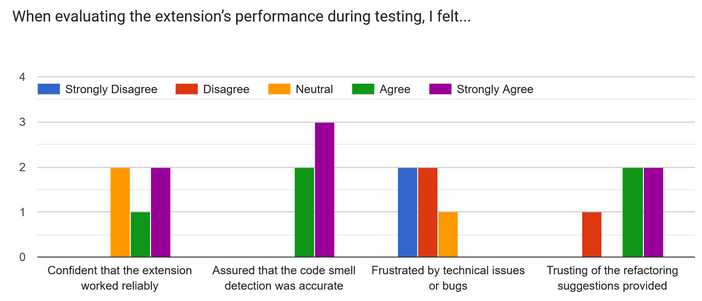
\includegraphics[width=0.7\textwidth]{../Images/usability-satisfaction-graph.png}
  \label{img:usability-satisfaction}
  \caption{User Satisfaction Survey Data}
\end{figure}

\subsection*{Qualitative Results}
Participants found the code smell detection intuitive and accurate, and they appreciated the preview feature and Accept/Reject buttons. However, they struggled with sidebar visibility, refactoring speed, and UI clarity. Hover descriptions were overwhelming, and some elements (e.g., ``(6/3)'') were unclear.

\section*{Discussion}
The usability test revealed that the extension performs well in detecting code smells and providing refactoring suggestions. Participants appreciated the energy savings feedback but requested clearer explanations of how refactoring improves energy efficiency. The sidebar and refactoring process were identified as major pain points, requiring immediate attention.\\

The extension met its core functionality objectives but fell short in UI clarity and performance reliability. Participants expressed interest in using the extension in the future, provided the identified issues are addressed. The test highlighted the need for better onboarding, clearer documentation, and performance optimizations to enhance user satisfaction and adoption.

\section*{Feedback and Implementation Plan}
The following table summarizes participant feedback and whether the suggested changes will be implemented:

\begin{table}[H]
\centering
\begin{tabular}{>{\raggedright\arraybackslash}p{6cm}p{3.2cm}>{\raggedright\arraybackslash}p{5cm}}
\toprule \textbf{Feedback} & \textbf{Implementation Decision} & \textbf{Reason} \\
\midrule
Relocate the sidebar or change its colour for better visibility. & Partial & The relocation of the sidebar is not something that is in scope during the development period. \\
Make Accept/Reject buttons more prominent and visually distinct. & Yes & High user frustration. \\
Allow users to customize colours for different types of smells. & Yes & Enhances user experience. \\
Optimize the refactoring process to reduce wait times. & No & This is a time intensive ask that is not in scope. \\
Add progress bars or loading messages to manage user expectations. & Yes & Additional messages will be added to the UI.\\
Provide step-by-step instructions and a tutorial for new users. & Yes & This was already planned and will be implemented for revision 1. \\
Simplify hover descriptions and provide examples or links to documentation. & Yes & The hover content will be improved for revision 1. \\
Explain how refactoring saves energy, possibly with visualizations. & Partial & No visualizations will be added, but better explanation of smells will be provided. \\
\bottomrule
\end{tabular}
\caption{Participant Feedback and Implementation Decisions}
\end{table}


\subsection{Performance}

This testing benchmarks the performance of ecooptimizer across 
files of varying sizes (250, 1000, and 3000 lines). The data includes detection times, 
refactoring times for specific smells, and energy measurement times. The goal is to 
identify scalability patterns, performance bottlenecks, and opportunities for optimization.\\

\textbf{Related Performance Requirement:} PR-1\\

\noindent The test cases for this module can be found \href{https://github.com/ssm-lab/capstone--source-code-optimizer/blob/new-poc/tests/benchmarking/benchmark.py}{here}\\

This script benchmarks the following components:

\begin{enumerate}
  \item \textbf{Detection/Analyzer Runtime} (via \texttt{AnalyzerController.run\_analysis})
  \item \textbf{Refactoring Runtime} (via \texttt{RefactorerController.run\_refactorer})
  \item \textbf{Energy Measurement Time} (via \texttt{CodeCarbonEnergyMeter.measure\_energy})
\end{enumerate}


For each detected smell (grouped by smell type), refactoring is run 10 times to compute average times.\\

\noindent The following is for your reference: \\

\begin{tabular}{|l|l|l|}
  \hline
  \textbf{Type of Smell} & \textbf{Code} & \textbf{Smell Name} \\
  \hline
  Pylint & R0913 & Long Parameter List \\
  Pylint & R6301 & No Self Use \\
  Pylint & R1729 & Use a Generator \\
  \hline
  Custom & LMC001 & Long Message Chain \\
  Custom & UVA001 & Unused Variable or Attribute \\
  Custom & LEC001 & Long Element Chain \\
  Custom & LLE001 & Long Lambda Expression \\
  Custom & SCL001 & String Concatenation in Loop \\
  Custom & CRC001 & Cache Repeated Calls \\
  \hline
\end{tabular}

\subsection*{1. Detection Time vs File Size}
\begin{figure}[H]
  \centering
  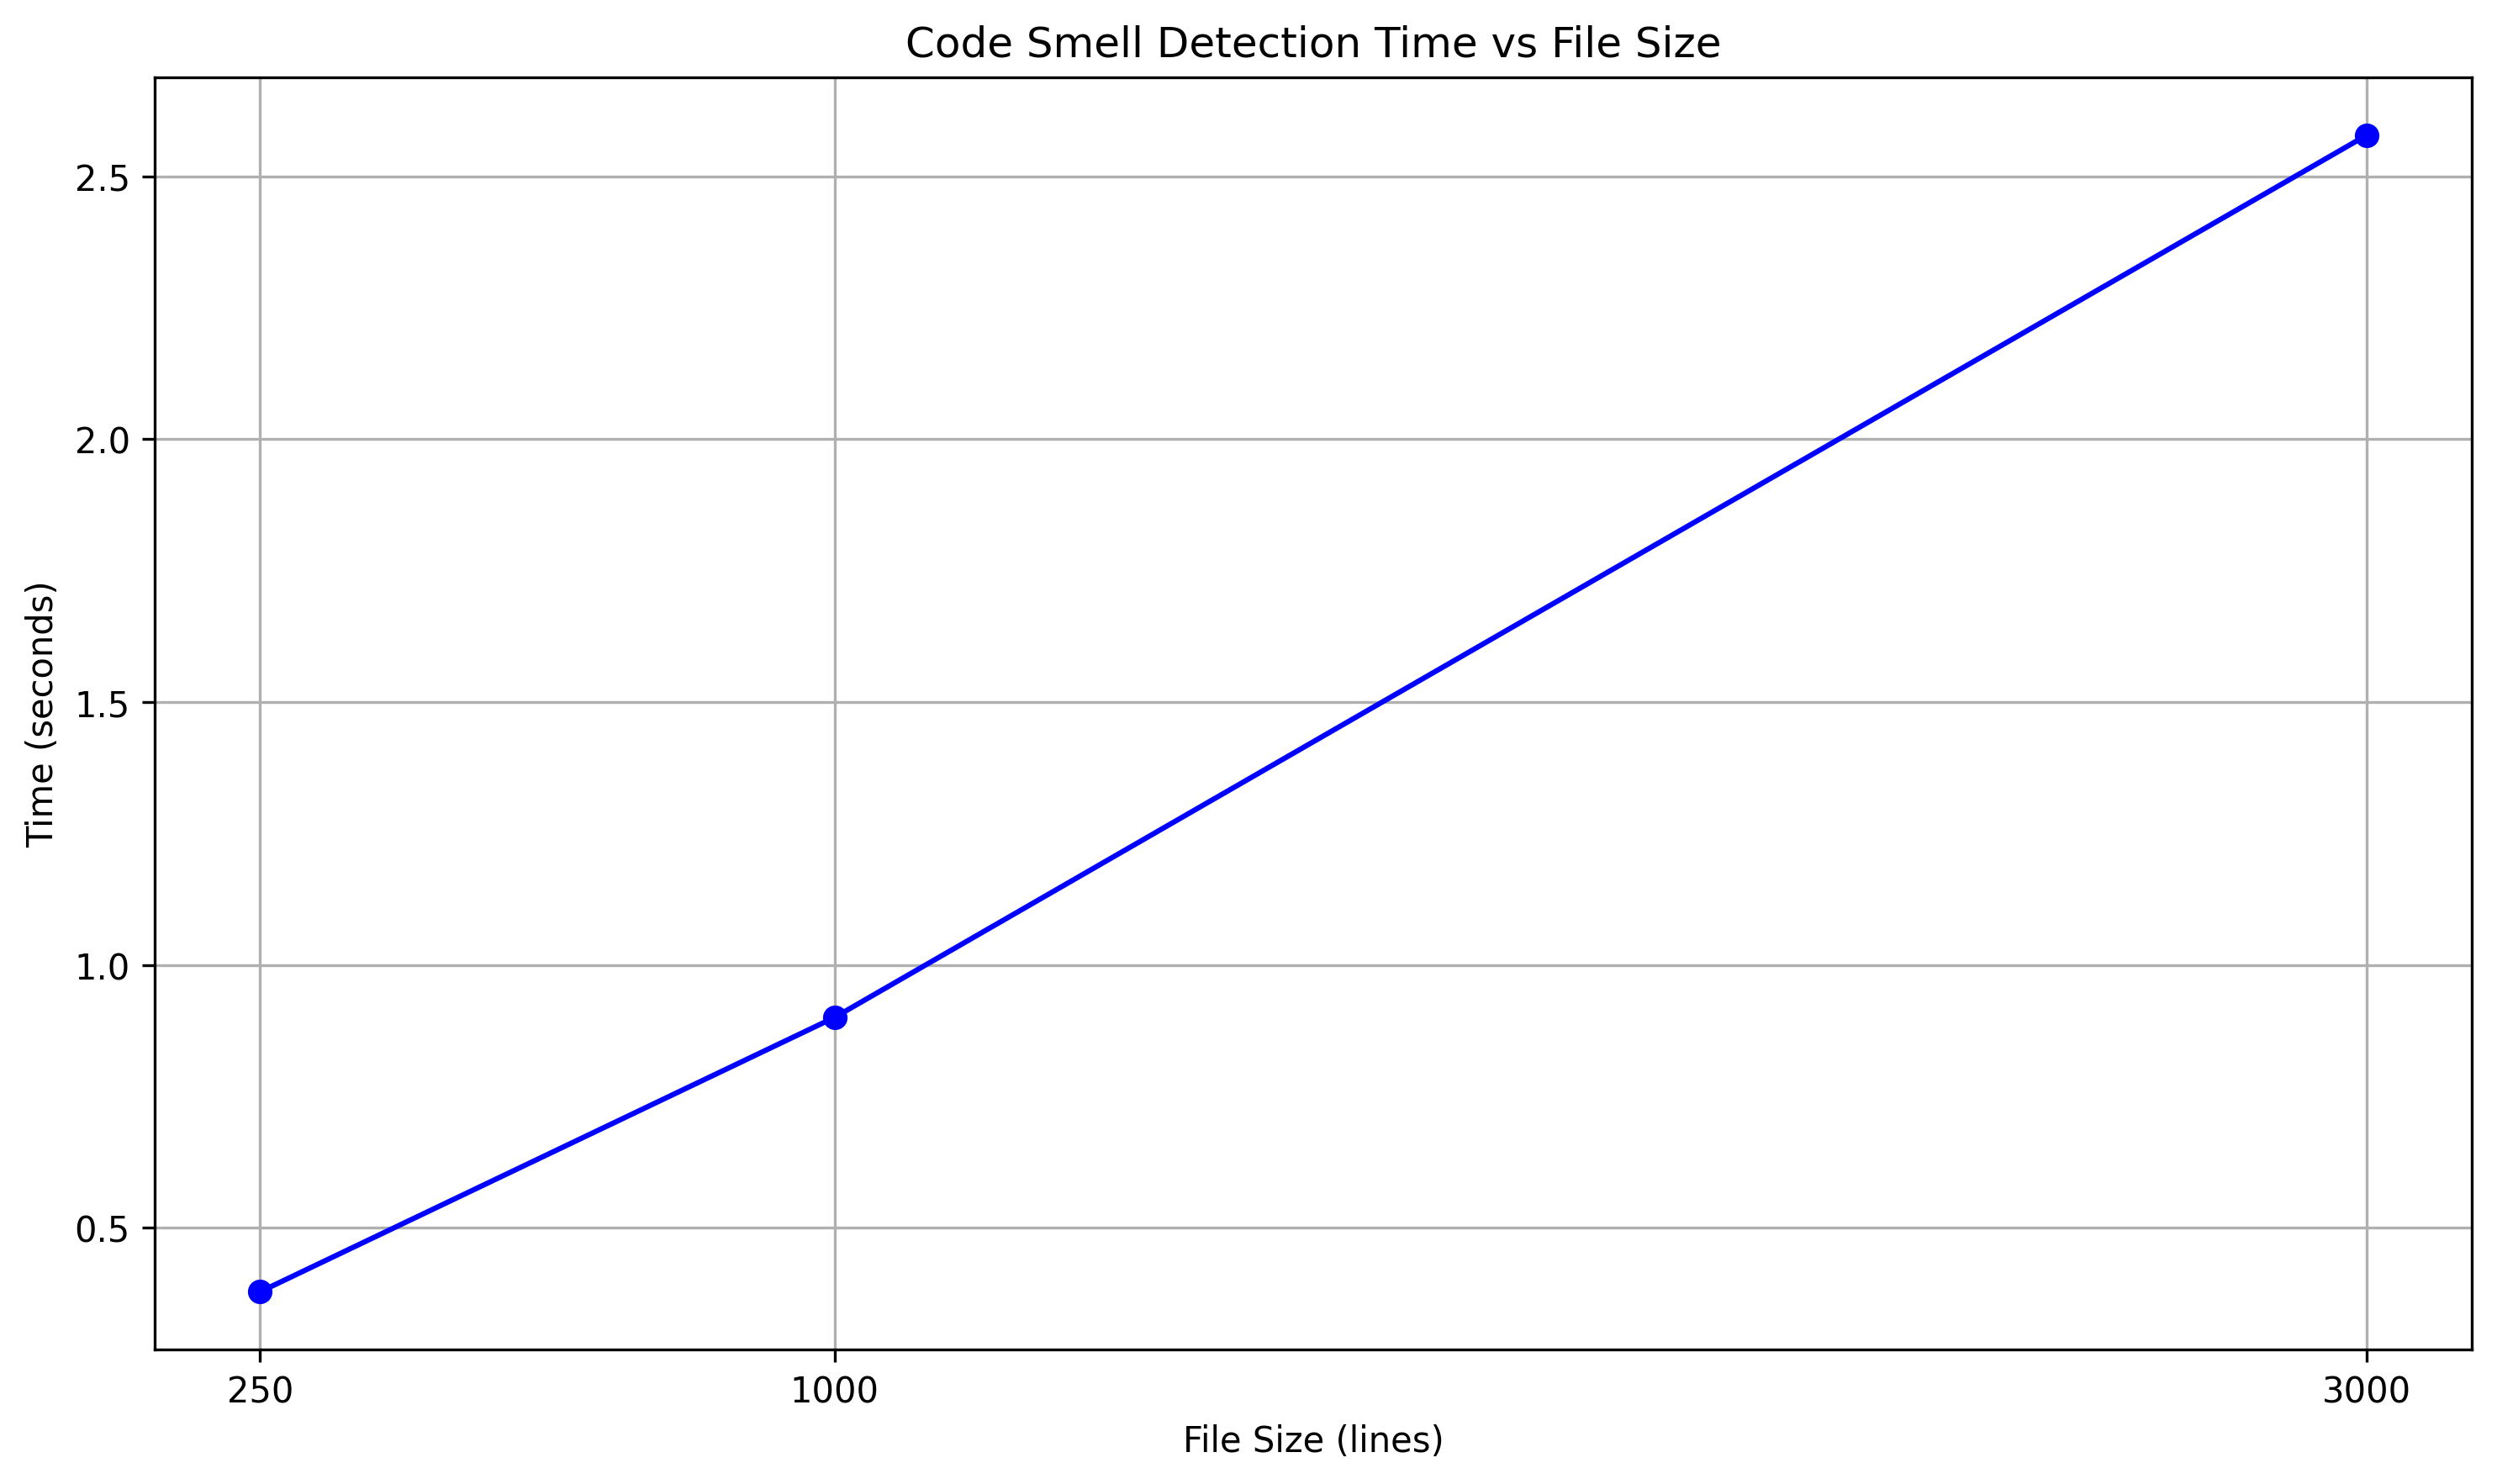
\includegraphics[width=\textwidth]{{../Images/detectionTimeVsFileSize.png}}
  \caption{Detection Time vs File Size}
\end{figure}

\noindent \textbf{What}: Linear plot showing code smell detection time growth with file size\\

\noindent \textbf{Why}: Understand scalability of detection mechanism\\

The detection time grows non-linearly with file size, suggesting a potential \(O(n^2)\) complexity. 
For a 250-line file, detection takes 0.38 seconds, while a 1000-line file takes 0.90 seconds (a 2.4× 
increase). At 3000 lines, the detection time jumps to 2.58 seconds (a 2.9× increase from 1000 lines). 
This indicates that the detection algorithm scales poorly for larger files, which could become 
problematic for very large codebases. However, the absolute times remain reasonable, with detection 
completing in under 3 seconds even for 3000-line files making this not a current critical bottleneck.

\subsection*{2. Refactoring Times by Smell Type (Log Scale)}
\begin{figure}[H]
    \centering
    \includegraphics[width=\textwidth]{../Images/refactoring\_times\_log\_scale.png}
    \caption{Refactoring Times by Smell Type (Log Scale)}
\end{figure}

\noindent \textbf{What}: Logarithmic plot of refactoring times per smell across file sizes\\

\noindent \textbf{Why}: Identify most expensive refactorings and scalability patterns\\

The logarithmic plot reveals a clear hierarchy of refactoring costs. The most expensive smells are \texttt{R6301} and \texttt{R0913}, which take 6.13 seconds and 5.65 seconds, respectively, for a 3000-line file. These smells show exponential growth, with \texttt{R6301} increasing by 14.6× from 250 to 3000 lines. In contrast, low-cost smells like \texttt{LLE001} and \texttt{LMC001} remain consistently fast (0.03 seconds) across all file sizes. This suggests that optimizing \texttt{R6301} and \texttt{R0913} should be a priority, as they dominate the refactoring time for larger files.

\subsection*{3. Refactoring Times Heatmap}
\begin{figure}[H]
    \centering
    \includegraphics[width=\textwidth]{../Images/refactoring\_times\_heatmap.png}
    \caption{Refactoring Times Heatmap}
\end{figure}

\noindent \textbf{What}: Color-coded matrix of refactoring times by smell/file size\\

\noindent \textbf{Why}: Quick visual identification of hot spots\\

The heatmap provides a quick visual summary of refactoring times across smells and file sizes. The darkest cells correspond to \texttt{R6301} and \texttt{R0913} at 3000 lines, confirming their status as the most expensive operations. In contrast, \texttt{LLE001} and \texttt{LMC001} remain light-colored across all sizes, indicating consistently low costs. The heatmap also highlights the dramatic variation in refactoring times: at 3000 lines, the fastest smell (\texttt{LLE001}) is 200× faster than the slowest (\texttt{R6301}).

\subsection*{4. Energy Measurement Times Distribution}
\begin{figure}[H]
    \centering
    \includegraphics[width=\textwidth]{../Images/energy\_measurement\_boxplot.png}
    \caption{Energy Measurement Times Distribution}
\end{figure}

\noindent \textbf{What}: Box plot of energy measurement durations\\

\noindent \textbf{Why}: Verify measurement consistency across operations\\

Energy measurement times are remarkably consistent, ranging from 5.54 to 6.14 seconds across all operations and file sizes. 
The box plot shows no significant variation with file size, suggesting that energy measurement is operation-specific 
rather than dependent on the size of the file. This stability could indicate that the energy measurement process has a fixed 
overhead, which could simplify efforts in the future if we were to create our own energy measurement module. 

\subsection*{5. Comparative Refactoring Times per File Size}
\begin{figure}[H]
    \centering
    \includegraphics[width=\textwidth]{../Images/refactoring\_times\_comparison.png}
    \caption{Comparative Refactoring Times per File Size}
\end{figure}

\noindent \textbf{What}: Side-by-side bar charts per file size\\

\noindent \textbf{Why}: Direct comparison of refactoring costs at different scales\\

The side-by-side bar charts reveal consistent dominance patterns across file sizes. \texttt{R6301} and \texttt{R0913} are always the top two most expensive smells, while \texttt{LLE001} and \texttt{LMC001} remain the cheapest. Notably, the relative cost difference between the most and least expensive smells increases with file size: at 250 lines, the ratio is 100:1, but at 3000 lines, it grows to 200:1. This suggests that the scalability of refactoring operations varies significantly by smell type.

\subsection*{6. Energy vs Refactoring Time Correlation}

\begin{figure}[H]
    \centering
    \includegraphics[width=\textwidth]{../Images/energy\_refactoring\_correlation.png}
    \caption{Energy vs Refactoring Time Correlation}
\end{figure}

\noindent \textbf{What}: Scatter plot comparing refactoring and energy measurement times\\

\noindent \textbf{Why}: Identify potential relationships between effort and energy impact\\

The scatter plot shows no clear correlation between refactoring time and energy measurement time. Fast refactorings like \texttt{LLE001} and slow refactorings like \texttt{R6301} both result in energy measurement times clustered between 5.5 and 6.1 seconds. This makes perfect sense as the refactoring operations and energy measurement are disjoint functionalities in the code. 

\subsection*{Key Insights and Recommendations}
\begin{itemize}
    \item \textbf{Bottleneck Identification:} The smells \texttt{R6301} and \texttt{R0913} are the primary bottlenecks, consuming over 50\% of the total refactoring time for 3000-line files. Optimizing these operations should be a top priority.
    \item \textbf{Scalability Concerns:} Both detection and refactoring times scale poorly with file size, suggesting \(O(n^2)\) complexity. This could become problematic for very large codebases.
    \item \textbf{Low-Hanging Fruit:} Smells like \texttt{LLE001} and \texttt{LMC001} are consistently fast to refactor, making them ideal candidates for early refactoring efforts.
    \item \textbf{Energy Measurement Stability:} Energy measurement times seem consistent across operations and file sizes, indicating a fixed overhead. This simplifies efforts to correlate refactoring with energy savings.
    \item \textbf{Disproportionate Costs:} The cost difference between the most and least expensive smells grows with file size, highlighting the need for targeted optimization.
\end{itemize}

The analysis reveals significant scalability challenges for both detection and refactoring, particularly for smells like \texttt{R6301} and \texttt{R0913}. While energy measurement times are stable, their lack of correlation with refactoring time suggests that additional metrics may be needed to accurately assess energy savings. Future work should focus on optimizing high-cost operations and improving the scalability of the detection algorithm.


\subsection{Maintainability and Support}
\begin{enumerate}

\item \textbf{test-MS-1: Extensibility for New Code Smells and Refactorings} \\[2mm]
To validate the extensibility of our tool, we structured the codebase using a modular design, where new code smell detection and refactoring functions can 
be easily added as separate components. In simpler terms, each refactoring and each custom detection is placed in its own file. A code walkthrough confirmed that 
existing modules remain unaffected when adding new detection logic. We successfully integrated a sample code smell and its corresponding refactoring method with 
minimal changes, ensuring that the new function was accessible through the main interface. This demonstrated that our architecture supports future expansions without 
disrupting core functionality.

\item \textbf{test-MS-2: Maintainable and Adaptable Codebase} \\[2mm]
We conducted a static analysis and documentation walkthrough to assess the maintainability of our codebase. The code was reviewed for modular organization, clear separation 
of concerns, and adherence to coding standards. All modules were correctly seperated and organzied. Documentation will be updated to include detailed descriptions of functions 
and configuration files, ensuring clarity for future developers. Code comments were refined to enhance readability, and function naming conventions were standardized for 
consistency. These efforts ensured that the tool remains adaptable to new Python versions and evolving best practices.

\item \textbf{test-MS-3: Easy rollback of updates in case of errors} \\[2mm]
Once releases are made, each release will be properly tagged and versioned to ensure smooth rollbacks through version control. This will all be handled with Git. done, but 
this approach guarantees that users will be able to revert to a previous stable version if needed, maintaining system integrity and minimizing disruptions.
\end{enumerate}


\subsection{Look and Feel}
\begin{enumerate}
\item \textbf{test-LF-1 Side-by-Side Code Comparison in IDE Plugin} \\[2mm]
The side-by-side code comparison feature in the IDE plugin was tested manually to verify that users can clearly view the original and refactored code within the VS Code interface. The test followed the procedure outlined in Test-LF-1, which specifies that upon initiating a refactoring operation, the plugin should display the original and modified versions of the code in parallel, allowing users to compare changes effectively.

The tester performed the test dynamically by opening a sample code file within the plugin and applying various refactoring operations across all detected code smells. The expected result was that the IDE plugin would correctly display the two versions side by side, with clear options for users to accept or reject each change. The actual result confirmed that the functionality operates as expected: refactored code was displayed adjacent to the original code, ensuring an intuitive comparison process. The tester was also able to interact with the accept/reject buttons, verifying their usability and correctness.

A screenshot of the successful test execution is provided in Figure \ref{fig:lf1_test}, illustrating the side-by-side code comparison functionality within the IDE plugin.

\FloatBarrier
\begin{figure}[h]
    \centering
    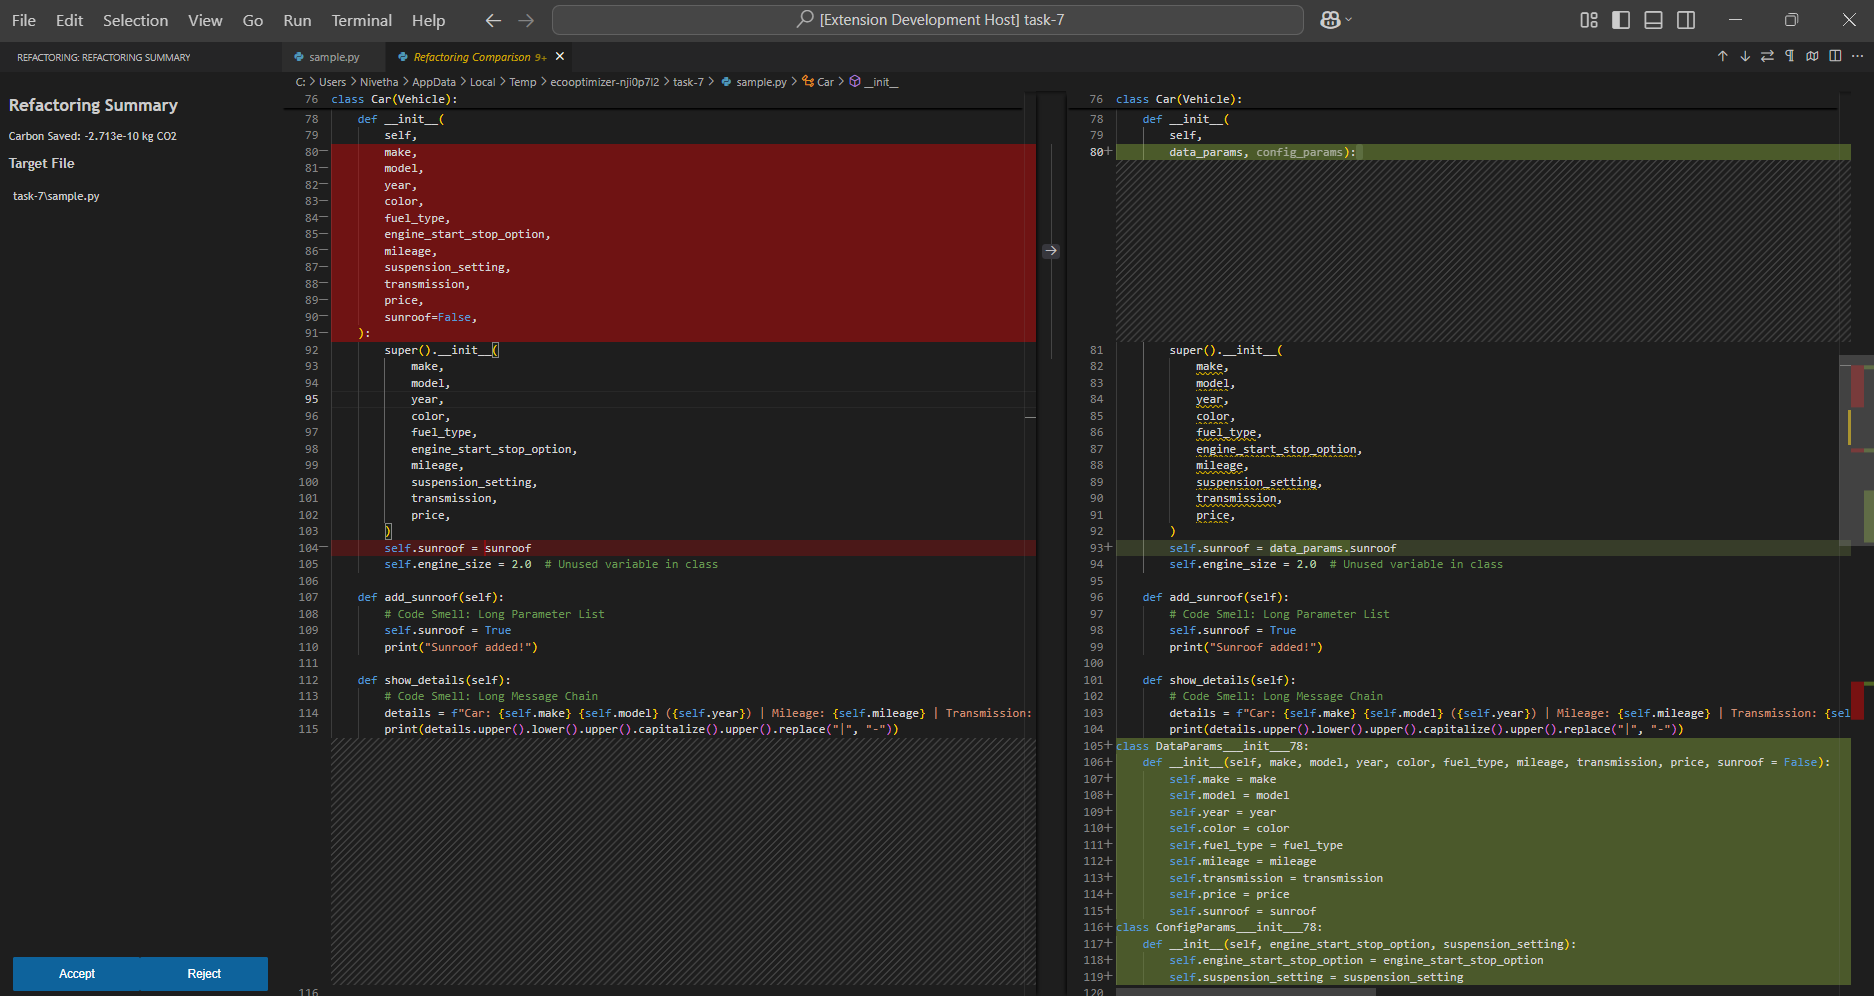
\includegraphics[width=0.8\linewidth]{../Images/test-LF-1-image.png}
    \caption{Side-by-Side Code Comparison in VS Code Plugin}
    \label{fig:lf1_test}
\end{figure}
\FloatBarrier 

\item \textbf{test-LF-2 Theme Adaptation in VS Code} \\[2mm]
The theme adaptation feature in the IDE plugin was tested manually to confirm that the plugin correctly adjusts to VS Code’s light and dark themes without requiring manual configuration. The tester performed the test by opening the plugin in both themes and switching between them using VS Code’s settings.

The expected result was that the plugin’s interface should automatically adjust when the theme is changed. The actual result confirmed that the plugin seamlessly transitioned between light and dark themes while maintaining a consistent interface. The images in Figures \ref{fig:lf2_light} and \ref{fig:lf2_dark} illustrate the side-by-side refactoring panel in both light mode and dark mode.

\FloatBarrier
\begin{figure}[h]
    \centering
    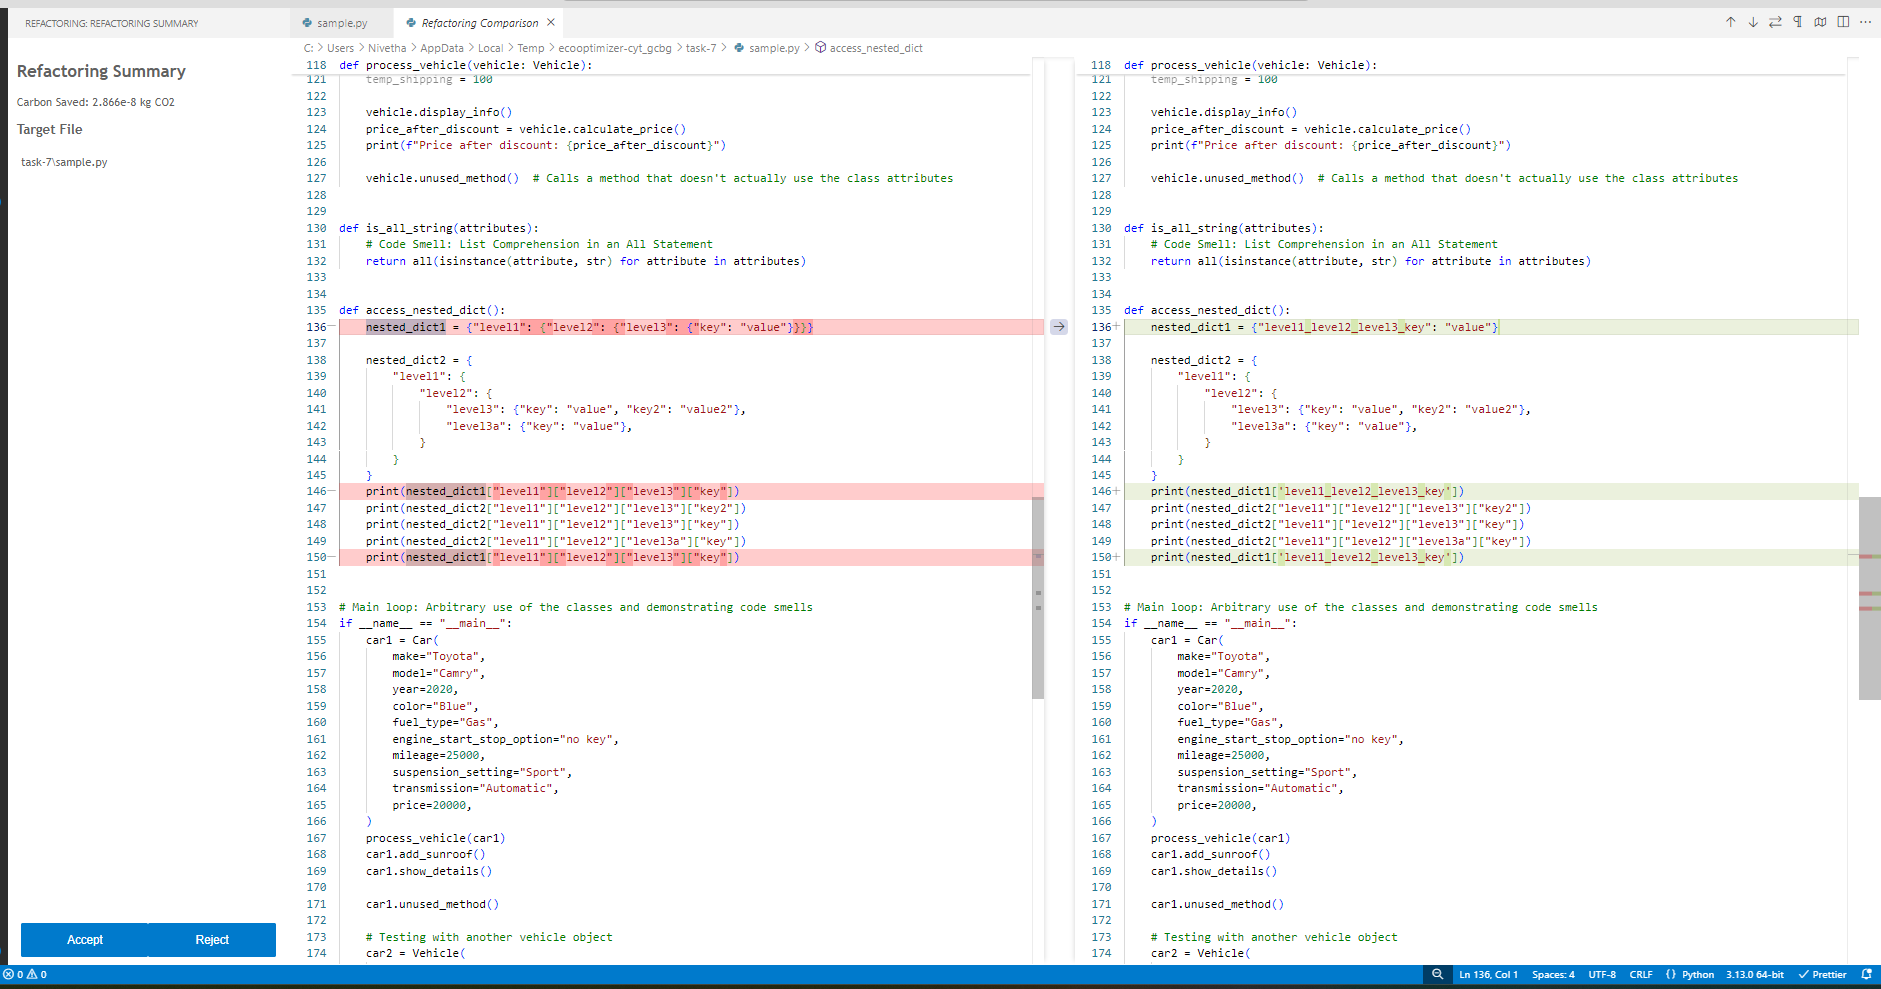
\includegraphics[width=0.8\linewidth]{../Images/test-LF-2-image-light.png}
    \caption{Side-by-Side Refactoring Panel in Light Mode}
    \label{fig:lf2_light}
\end{figure}
\FloatBarrier 

\FloatBarrier 
\begin{figure}[h]
    \centering
    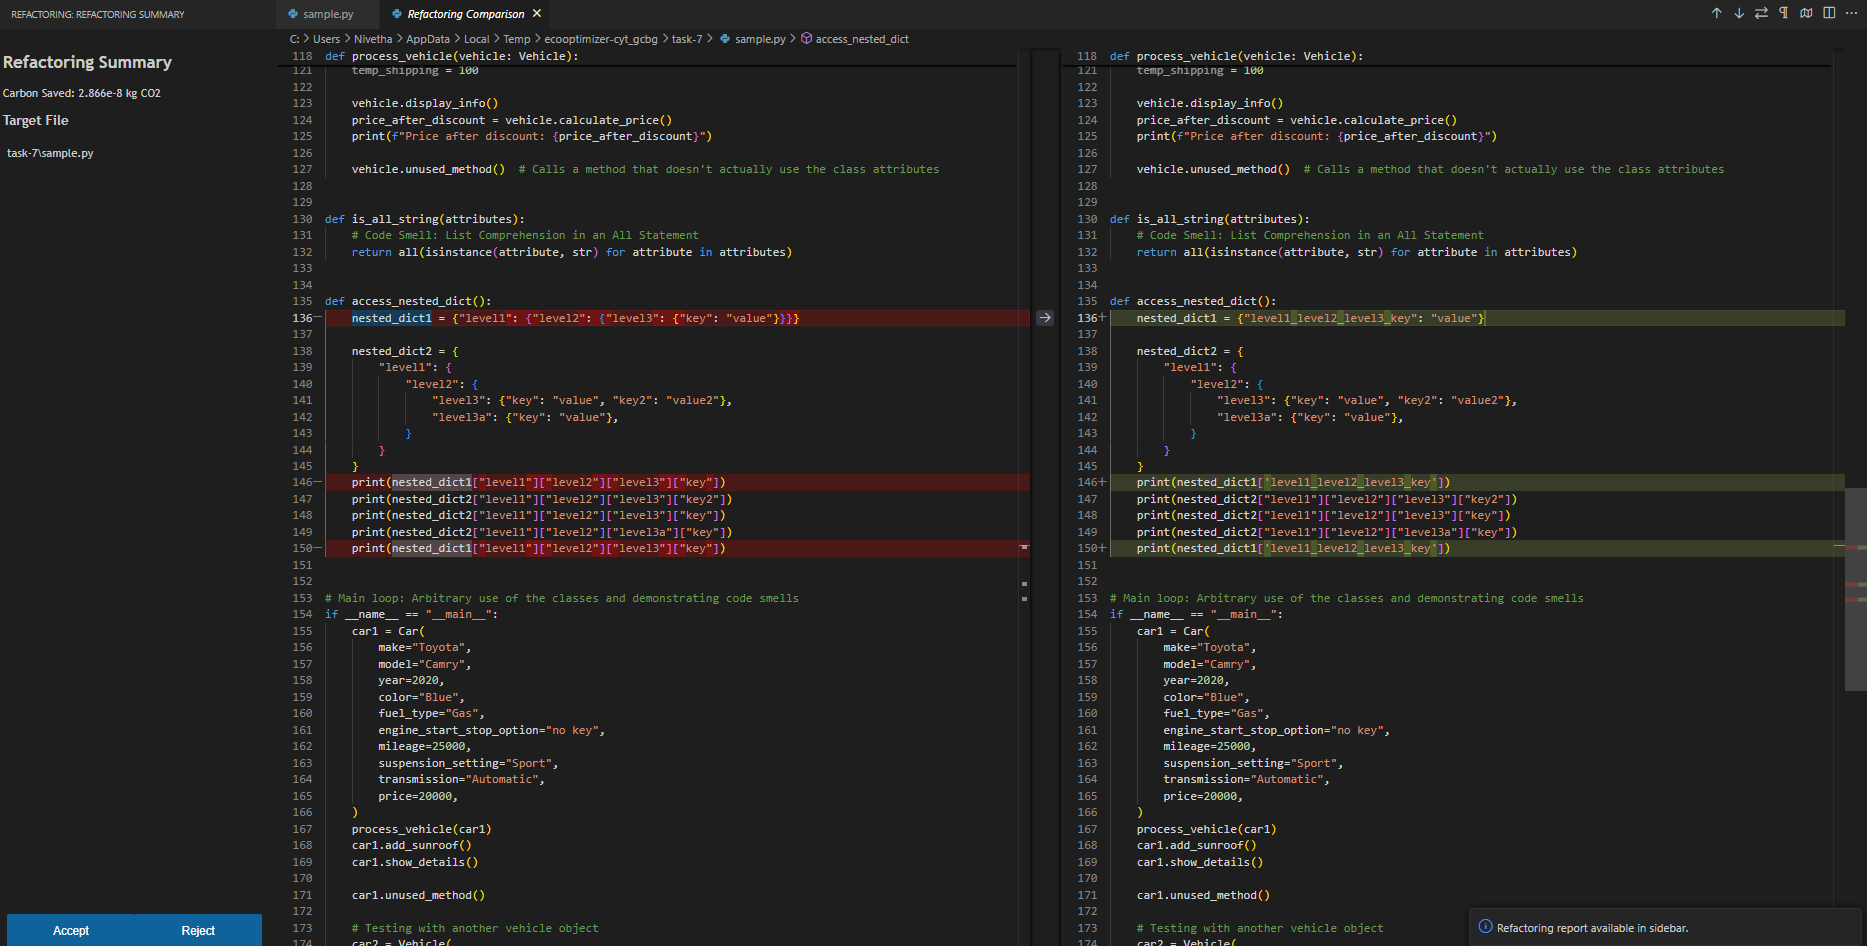
\includegraphics[width=0.8\linewidth]{../Images/test-LF-2-image-dark.png}
    \caption{Side-by-Side Refactoring Panel in Dark Mode}
    \label{fig:lf2_dark}
\end{figure}
\FloatBarrier 

\item \textbf{test-LF-3 Design Acceptance} \\[2mm]
The design acceptance test was conducted as part of the usability testing session, where developers and testers interacted with the plugin and provided feedback. This test evaluated user experience, ease of navigation, and overall satisfaction with the plugin’s interface.

The expected result was that users would be able to interact with the plugin smoothly and provide structured feedback. The actual result confirmed that users were able to navigate and use the plugin effectively. The feedback collected during this session was used to assess the overall usability of the plugin. More details regarding this evaluation can be found in the Usability Testing section.

\end{enumerate}


\section{Comparison to Existing Implementation}	

This section will not be appropriate for every project.

\section{Unit Testing}
\newcounter{testcase}
\newcommand{\testcount}{\stepcounter{testcase}\thetestcase}
\renewcommand{\arraystretch}{1.2} % Adjust row height for better readability

\subsection{API Endpoints}

\subsubsection{Smell Detection Endpoint}

\begin{longtable}{c 
  >{\raggedright\arraybackslash}p{1.5cm} 
  >{\raggedright\arraybackslash}p{4.5cm} 
  >{\raggedright\arraybackslash}p{4cm} 
  >{\raggedright\arraybackslash}p{3cm} c}
  \toprule
  \textbf{ID} & \textbf{Ref. Req.} & \textbf{Action} & \textbf{Expected Result} & \textbf{Actual Result} & \textbf{Result} \\ 
  \midrule
  \endfirsthead

  \multicolumn{6}{l}{\textit{(Continued from previous page)}} \\ 
  \toprule
  \textbf{ID} & \textbf{Ref. Req.} & \textbf{Action} & \textbf{Expected Result} & \textbf{Actual Result} & \textbf{Result} \\ 
  \midrule
  \endhead

  \multicolumn{6}{r}{\textit{Continued on next page}} \\
  \endfoot

  \bottomrule
  \caption{Smell Detection Endpoint Test Cases}
  \label{table:detection_endpoint_tests}
  \endlastfoot

  TC\testcount & FR10, OER-IAS1 & User requests to detect smells in a valid file. & Status code is 200. Response contains 2 smells. & All assertions pass. & \cellcolor{green} Pass \\ \midrule
  TC\testcount & FR10, OER-IAS1 & User requests to detect smells in a non-existent file. & Status code is 404. Error message indicates file not found. & All assertions pass. & \cellcolor{green} Pass \\ \midrule
  TC\testcount & FR10, OER-IAS1 & Internal server error occurs during smell detection. & Status code is 500. Error message indicates internal server error. & All assertions pass. & \cellcolor{green} Pass \\ 
\end{longtable}

\subsubsection{Refactor Endpoint}

\begin{longtable}{c 
  >{\raggedright\arraybackslash}p{1.5cm} 
  >{\raggedright\arraybackslash}p{4.5cm} 
  >{\raggedright\arraybackslash}p{4cm} 
  >{\raggedright\arraybackslash}p{3cm} c}
  \toprule
  \textbf{ID} & \textbf{Ref. Req.} & \textbf{Action} & \textbf{Expected Result} & \textbf{Actual Result} & \textbf{Result} \\ 
  \midrule
  \endfirsthead

  \multicolumn{6}{l}{\textit{(Continued from previous page)}} \\ 
  \toprule
  \textbf{ID} & \textbf{Ref. Req.} & \textbf{Action} & \textbf{Expected Result} & \textbf{Actual Result} & \textbf{Result} \\ 
  \midrule
  \endhead

  \multicolumn{6}{r}{\textit{Continued on next page}} \\
  \endfoot

  \bottomrule
  \caption{Refactor Endpoint Test Cases}
  \label{table:refactor_endpoint_tests}
  \endlastfoot

  TC\testcount & FR10, OER-IAS1 & User requests to refactor a valid source directory. & Status code is 200. Response contains refactored data and updated smells. & All assertions pass. & \cellcolor{green} Pass \\ \midrule
  TC\testcount & FR10, OER-IAS1 & User requests to refactor a non-existent source directory. & Status code is 404. Error message indicates directory not found. & All assertions pass. & \cellcolor{green} Pass \\ \midrule 
  TC\testcount & FR10, OER-IAS1 & Energy is not saved after refactoring. & Status code is 400. Error message indicates energy was not saved. & All assertions pass. & \cellcolor{green} Pass \\ \midrule 
  TC\testcount & FR10, OER-IAS1 & Initial energy measurement fails. & Status code is 400. Error message indicates initial emissions could not be retrieved. & All assertions pass. & \cellcolor{green} Pass \\ \midrule 
  TC\testcount & FR10, OER-IAS1 & Final energy measurement fails. & Status code is 400. Error message indicates final emissions could not be retrieved. & All assertions pass. & \cellcolor{green} Pass \\ \midrule 
  TC\testcount & FR10, OER-IAS1 & Unexpected error occurs during refactoring. & Status code is 400. Error message contains the exception details. & All assertions pass. & \cellcolor{green} Pass \\ 
\end{longtable}

\subsection{Analyzer Controller Module}

\begin{longtable}{c 
  >{\raggedright\arraybackslash}p{1.5cm} 
  >{\raggedright\arraybackslash}p{4.5cm} 
  >{\raggedright\arraybackslash}p{4cm} 
  >{\raggedright\arraybackslash}p{3cm} c}
  \toprule
  \textbf{ID} & \textbf{Ref. Req.} & \textbf{Action} & \textbf{Expected Result} & \textbf{Actual Result} & \textbf{Result} \\ 
  \midrule
  \endfirsthead

  \multicolumn{6}{l}{\textit{(Continued from previous page)}} \\ 
  \toprule
  \textbf{ID} & \textbf{Ref. Req.} & \textbf{Action} & \textbf{Expected Result} & \textbf{Actual Result} & \textbf{Result} \\ 
  \midrule
  \endhead

  \multicolumn{6}{r}{\textit{Continued on next page}} \\
  \endfoot

  \bottomrule
  \caption{Analyzer Controller Module Test Cases}
  \label{table:analyzer_controller_tests}
  \endlastfoot

  TC\testcount & FR2, FR5, PR-PAR3 & Test detection of repeated function calls in AST-based analysis. & One repeated function call should be detected. & All assertions pass. & \cellcolor{green} Pass \\ \midrule
  TC\testcount & FR2, FR5, PR-PAR3 & Test detection of repeated method calls on the same object instance. & One repeated method call should be detected. & All assertions pass. & \cellcolor{green} Pass \\ \midrule
  TC\testcount & FR2 & Test that no code smells are detected in a clean file. & The system should return an empty list of smells. & All assertions pass. & \cellcolor{green} Pass \\ \midrule
  TC\testcount & FR2, PR-PAR2 & Test filtering of smells by analysis method. & The function should return only smells matching the specified method (AST, Pylint, Astroid). & All assertions pass. & \cellcolor{green} Pass \\ \midrule
  TC\testcount & FR2, PR-PAR2 & Test generating custom analysis options for AST-based analysis. & The generated options should include callable detection functions. & All assertions pass. & \cellcolor{green} Pass \\ \midrule
  TC\testcount & FR2, FR5, PR-PAR3 & Test correct logging of detected code smells. & Detected smells should be logged with correct details. & All assertions pass. & \cellcolor{green} Pass \\ \midrule
  TC\testcount & FR2, FR5 & Test handling of an empty registry when filtering smells. & The function should return an empty dictionary. & All assertions pass. & \cellcolor{green} Pass \\ \midrule
  TC\testcount & FR2, PR-PAR2 & Test that smells remain unchanged if no modifications occur. & The function should not modify existing smells if no changes are detected. & All assertions pass. & \cellcolor{green} Pass \\ 
\end{longtable}



\subsection{CodeCarbon Measurement}

\begin{longtable}{c 
  >{\raggedright\arraybackslash}p{1.5cm} 
  >{\raggedright\arraybackslash}p{4.5cm} 
  >{\raggedright\arraybackslash}p{4cm} 
  >{\raggedright\arraybackslash}p{3cm} c}
  \toprule
  \textbf{ID} & \textbf{Ref. Req.} & \textbf{Action} & \textbf{Expected Result} & \textbf{Actual Result} & \textbf{Result} \\ 
  \midrule
  \endfirsthead

  \multicolumn{6}{l}{\textit{(Continued from previous page)}} \\ 
  \toprule
  \textbf{ID} & \textbf{Ref. Req.} & \textbf{Action} & \textbf{Expected Result} & \textbf{Actual Result} & \textbf{Result} \\ 
  \midrule
  \endhead

  \multicolumn{6}{r}{\textit{Continued on next page}} \\
  \endfoot

  \bottomrule
  \caption{CodeCarbon Measurement Test Cases}
  \label{table:measurement_tests}
  \endlastfoot

  TC\testcount & PR-RFT1, FR6 & Trigger CodeCarbon measurements with a valid file path. & CodeCarbon subprocess for the file should be invoked at least once. \texttt{EmissionsTracker. start} and \texttt{stop} API endpoints should be called. Success message ``CodeCarbon measurement completed successfully." should be logged. & All assertions pass. & \cellcolor{green} Pass \\ 
  \midrule
  TC\testcount & PR-RFT1 & Trigger CodeCarbon function with a valid file path that causes a subprocess failure. & CodeCarbon subprocess run should still be invoked. \texttt{EmissionsTracker. start} and \texttt{stop} API endpoints should be called. An error message ``Error executing file" should be logged. Returned emissions data should be \texttt{None} since the execution failed.& All assertions pass. & \cellcolor{green} Pass \\ 
  \midrule
  TC\testcount & FR5, PR-SCR1 & Results produced by CodeCarbon run are at a valid CSV file path and can be read. & Emissions data should be read successfully from the CSV file. The function should return the last row of emissions data. & All assertions pass. & \cellcolor{green} Pass \\ 
  \midrule
  TC\testcount & PR-RFT1, FR6 & Results produced by CodeCarbon run are at a valid CSV file path but the file cannot be read. & An error message ``Error reading file" should be logged. The function should return \texttt{None} because the file reading failed. & All assertions pass. & \cellcolor{green} Pass \\ 
   \midrule
  TC\testcount & PR-RFT1, FR5 & Given CSV Path for results produced by CodeCarbon does not have a file. & An error message ``File \texttt{file path} does not exist." should be logged.The function should return \texttt{None} since the file does not exist. & All assertions pass. & \cellcolor{green} Pass \\ 
\end{longtable}

\subsection{Smell Analyzers}

\subsubsection{String Concatenation in Loop}

\begin{longtable}{c 
  >{\raggedright\arraybackslash}p{1.5cm} 
  >{\raggedright\arraybackslash}p{4.5cm} 
  >{\raggedright\arraybackslash}p{4cm} 
  >{\raggedright\arraybackslash}p{3cm} c}
  \toprule
  \textbf{ID} & \textbf{Ref. Req.} & \textbf{Action} & \textbf{Expected Result} & \textbf{Actual Result} & \textbf{Result} \\ 
  \midrule
  \endfirsthead

  \multicolumn{6}{l}{\textit{(Continued from previous page)}} \\ 
  \toprule
  \textbf{ID} & \textbf{Ref. Req.} & \textbf{Action} & \textbf{Expected Result} & \textbf{Actual Result} & \textbf{Result} \\ 
  \midrule
  \endhead

  \multicolumn{6}{r}{\textit{Continued on next page}} \\
  \endfoot

  \bottomrule
  \caption{String Concatenation in Loop Detection Test Cases}
  \label{table:string_concat_detection_tests}
  \endlastfoot

  TC\testcount & FR2 & Detects \texttt{+=} string concatenation inside a \texttt{for} loop. & One smell detected with target \texttt{result} and line 4. & All assertions pass. & \cellcolor{green} Pass \\ 
  \midrule
  TC\testcount & FR2 & Detects \texttt{<var = var + ...>} string concatenation inside a loop. & One smell detected with target \texttt{result} and line 4. & All assertions pass. & \cellcolor{green} Pass \\ 
  \midrule
  TC\testcount & FR2 & Detects \texttt{+=} string concatenation inside a \texttt{while} loop. & One smell detected with target \texttt{result} and line 4. & All assertions pass. & \cellcolor{green} Pass \\ 
  \midrule
  TC\testcount & FR2 & Detects \texttt{+=} modifying a list item inside a loop. & One smell detected with target \lstinline|self.text[0]| and line 6. & All assertions pass. & \cellcolor{green} Pass \\ 
  \midrule
  TC\testcount & FR2 & Detects \texttt{+=} modifying an object attribute inside a loop. & One smell detected with target \lstinline|self.text| and line 6. & All assertions pass. & \cellcolor{green} Pass \\ 
  \midrule
  TC\testcount & FR2 & Detects \texttt{+=} modifying a dictionary value inside a loop. & One smell detected with target \texttt{data['key']} and line 4. & All assertions pass. & \cellcolor{green} Pass \\ 
  \midrule
  TC\testcount & FR2 & Detects multiple separate string concatenations in a loop. & Two smells detected with targets \texttt{result} and \texttt{logs[0]} on line 5. & All assertions pass. & \cellcolor{green} Pass \\ 
  \midrule
  TC\testcount & FR2 & Detects string concatenations with re-assignments inside the loop. & One smell detected with target \texttt{result} and line 4. & All assertions pass. & \cellcolor{green} Pass \\ 
  \midrule
  TC\testcount & FR2 & Detects concatenation inside nested loops. & One smell detected with target \texttt{result} and line 5. & All assertions pass. & \cellcolor{green} Pass \\ 
  \midrule
  TC\testcount & FR2 & Detects multi-level concatenations belonging to the same smell. & One smell detected with target \texttt{result} and two occurrences on lines 4 and 5. & All assertions pass. & \cellcolor{green} Pass \\ 
  \midrule
  TC\testcount & FR2 & Detects \texttt{+=} inside an \texttt{if-else} condition within a loop. & One smell detected with target \texttt{result} and two occurrences on line 4. & All assertions pass. & \cellcolor{green} Pass \\ 
  \midrule
  TC\testcount & FR2 & Detects \texttt{+=} using f-strings inside a loop. & One smell detected with target \texttt{result} and line 4. & All assertions pass. & \cellcolor{green} Pass \\ 
  \midrule
  TC\testcount & FR2 & Detects \texttt{+=} using \texttt{\%} formatting inside a loop. & One smell detected with target \texttt{result} and line 4. & All assertions pass. & \cellcolor{green} Pass \\ 
  \midrule
  TC\testcount & FR2 & Detects \texttt{+=} using \texttt{.format()} inside a loop. & One smell detected with target \texttt{result} and line 4. & All assertions pass. & \cellcolor{green} Pass \\ 
  \midrule
  TC\testcount & FR2 & Ensures accessing the concatenation variable inside the loop is NOT flagged. & No smells detected. & All assertions pass. & \cellcolor{green} Pass \\ 
  \midrule
  TC\testcount & FR2 & Ensures regular string assignments are NOT flagged. & No smells detected. & All assertions pass. & \cellcolor{green} Pass \\ 
  \midrule
  TC\testcount & FR2 & Ensures number operations with \texttt{+=} are NOT flagged. & No smells detected. & All assertions pass. & \cellcolor{green} Pass \\ 
  \midrule
  TC\testcount & FR2 & Ensures string concatenation OUTSIDE a loop is NOT flagged. & No smells detected. & All assertions pass. & \cellcolor{green} Pass \\ 
  \midrule
  TC\testcount & FR2 & Detects a variable concatenated multiple times in the same loop iteration. & One smell detected with target \texttt{result} and two occurrences on line 4. & All assertions pass. & \cellcolor{green} Pass \\ 
  \midrule
  TC\testcount & FR2 & Detects concatenation where both prefix and suffix are added. & One smell detected with target \texttt{result} and line 4. & All assertions pass. & \cellcolor{green} Pass \\ 
  \midrule
  TC\testcount & FR2 & Detects \texttt{+=} where new values are inserted at the beginning instead of the end. & One smell detected with target \texttt{result} and line 4. & All assertions pass. & \cellcolor{green} Pass \\ 
  \midrule
  TC\testcount & FR2 & Ignores potential smells where type cannot be confirmed as a string. & No smells detected. & All assertions pass. & \cellcolor{green} Pass \\ 
  \midrule
  TC\testcount & FR2 & Detects string concatenation where type is inferred from function type hints. & One smell detected with target \texttt{result} and line 4. & All assertions pass. & \cellcolor{green} Pass \\ 
  \midrule
  TC\testcount & FR2 & Detects string concatenation where type is inferred from variable type hints. & One smell detected with target \texttt{result} and line 4. & All assertions pass. & \cellcolor{green} Pass \\ 
  \midrule
  TC\testcount & FR2 & Detects string concatenation where type is inferred from class attributes. & One smell detected with target \texttt{result} and line 9. & All assertions pass. & \cellcolor{green} Pass \\ 
  \midrule
  TC\testcount & FR2 & Detects string concatenation where type is inferred from the initial value assigned. & One smell detected with target \texttt{result} and line 4. & All assertions pass. & \cellcolor{green} Pass \\ 
\end{longtable}

\subsubsection{Long Element Chain Detector Module}

\begin{longtable}{c 
  >{\raggedright\arraybackslash}p{1.5cm} 
  >{\raggedright\arraybackslash}p{4.5cm} 
  >{\raggedright\arraybackslash}p{4cm} 
  >{\raggedright\arraybackslash}p{3cm} c}
  \toprule
  \textbf{ID} & \textbf{Ref. Req.} & \textbf{Action} & \textbf{Expected Result} & \textbf{Actual Result} & \textbf{Result} \\ 
  \midrule
  \endfirsthead

  \multicolumn{6}{l}{\textit{(Continued from previous page)}} \\ 
  \toprule
  \textbf{ID} & \textbf{Ref. Req.} & \textbf{Action} & \textbf{Expected Result} & \textbf{Actual Result} & \textbf{Result} \\ 
  \midrule
  \endhead

  \multicolumn{6}{r}{\textit{Continued on next page}} \\
  \endfoot

  \bottomrule
  \caption{Long Element Chain Detector Module Test Cases}
  \label{table:lec_tests}
  \endlastfoot

  TC\testcount & FR2 & Test with code that has no chains. & No chains should be detected. & All assertions pass. & \cellcolor{green} Pass \\ \midrule
  TC\testcount & FR2 & Test with chains shorter than threshold. & No chains should be detected for threshold of 5. & All assertions pass. & \cellcolor{green} Pass \\ \midrule
  TC\testcount & FR2  & Test with chains exactly at threshold. & One chain should be detected at line 3. & All assertions pass. & \cellcolor{green} Pass \\ \midrule
  TC\testcount & FR2 & Test with chains longer than threshold. & One chain should be detected with message ``Dictionary chain too long (4/3)''. & All assertions pass. & \cellcolor{green} Pass \\ \midrule
  TC\testcount & FR2 & Test with multiple chains in the same file. & Two chains should be detected at different lines. & All assertions pass. & \cellcolor{green} Pass \\ \midrule
  TC\testcount & FR2 & Test chains inside nested functions and classes. & Two chains should be detected, one inside a function, one inside a class. & All assertions pass. & \cellcolor{green} Pass \\ \midrule
  TC\testcount & FR2 & Test that chains on the same line are reported only once. & One chain should be detected at line 4. & All assertions pass. & \cellcolor{green} Pass \\ \midrule
  TC\testcount & FR2 & Test chains with different variable types. & Two chains should be detected, one in a list and one in a tuple. & All assertions pass. & \cellcolor{green} Pass \\ \midrule
  TC\testcount & FR2 & Test with a custom threshold value. & No chains detected with threshold 4. One chain detected with threshold 2. & All assertions pass. & \cellcolor{green} Pass \\ \midrule
  DLEC10 & FR2 & Test the structure of the returned LECSmell object. & Object should have correct type, path, module, symbol, and occurrence details. & All assertions pass. & \cellcolor{green} Pass \\ \midrule
  DLEC11 & FR2 & Test chains within complex expressions. & Three chains should be detected in different contexts. & All assertions pass. & \cellcolor{green} Pass \\ \midrule
  DLEC12 & FR2 & Test with an empty file. & No chains should be detected. & All assertions pass. & \cellcolor{green} Pass \\ \midrule
  DLEC13 & FR2 & Test with threshold of 1 (every subscript reported). & One chain should be detected with message ``Dictionary chain too long (5/5)''. & All assertions pass. & \cellcolor{green} Pass \\
\end{longtable}

\subsubsection{Repeated Calls Detection Module}

\begin{longtable}{c 
  >{\raggedright\arraybackslash}p{1.5cm} 
  >{\raggedright\arraybackslash}p{4.5cm} 
  >{\raggedright\arraybackslash}p{4cm} 
  >{\raggedright\arraybackslash}p{3cm} c}
  \toprule
  \textbf{ID} & \textbf{Ref. Req.} & \textbf{Action} & \textbf{Expected Result} & \textbf{Actual Result} & \textbf{Result} \\ 
  \midrule
  \endfirsthead

  \multicolumn{6}{l}{\textit{(Continued from previous page)}} \\ 
  \toprule
  \textbf{ID} & \textbf{Ref. Req.} & \textbf{Action} & \textbf{Expected Result} & \textbf{Actual Result} & \textbf{Result} \\ 
  \midrule
  \endhead

  \multicolumn{6}{r}{\textit{Continued on next page}} \\
  \endfoot

  \bottomrule
  \caption{Repeated Calls Detection Module Test Cases}
  \label{table:crc_tests}
  \endlastfoot

  TC\testcount & FR2, PR-PAR2 & Test detection of repeated function calls within the same scope. & One repeated call detected with two occurrences. & All assertions pass. & \cellcolor{green} Pass \\ \midrule
  TC\testcount & FR2, PR-PAR2 & Test detection of repeated method calls on the same object instance. & One repeated method call detected with two occurrences. & All assertions pass. & \cellcolor{green} Pass \\ \midrule
  TC\testcount & FR2 & Test that function calls with different arguments are not flagged. & No repeated calls should be detected. & All assertions pass. & \cellcolor{green} Pass \\ \midrule
  TC\testcount & FR2 & Test that function calls on modified objects are not flagged. & No repeated calls should be detected due to object state change. & All assertions pass. & \cellcolor{green} Pass \\ \midrule
  TC\testcount & FR2, PR-PAR3 & Test detection of repeated external function calls. & One repeated function call detected with two occurrences. & All assertions pass. & \cellcolor{green} Pass \\ \midrule
  TC\testcount & FR2, PR-PAR3 & Test detection of repeated calls to expensive built-in functions. & One repeated function call detected with two occurrences. & All assertions pass. & \cellcolor{green} Pass \\ \midrule
  TC\testcount & FR2, PR-PAR3 & Test that built-in functions with primitive arguments are not flagged. & No repeated calls should be detected. & All assertions pass. & \cellcolor{green} Pass \\ \midrule
  TC\testcount & FR2 & Test that method calls on different object instances are not flagged. & No repeated calls should be detected. & All assertions pass. & \cellcolor{green} Pass \\ 
\end{longtable}

\subsubsection{Long Lambda Element Detection Module}

\begin{longtable}{c 
  >{\raggedright\arraybackslash}p{1.5cm} 
  >{\raggedright\arraybackslash}p{4.5cm} 
  >{\raggedright\arraybackslash}p{4cm} 
  >{\raggedright\arraybackslash}p{3cm} c}
  \toprule
  \textbf{ID} & \textbf{Ref. Req.} & \textbf{Action} & \textbf{Expected Result} & \textbf{Actual Result} & \textbf{Result} \\ 
  \midrule
  \endfirsthead

  \multicolumn{6}{l}{\textit{(Continued from previous page)}} \\ 
  \toprule
  \textbf{ID} & \textbf{Ref. Req.} & \textbf{Action} & \textbf{Expected Result} & \textbf{Actual Result} & \textbf{Result} \\ 
  \midrule
  \endhead

  \multicolumn{6}{r}{\textit{Continued on next page}} \\
  \endfoot

  \bottomrule
  \caption{Long Lambda Element Detector Module Test Cases}
  \label{table:lle_tests}
  \endlastfoot

  TC\testcount & FR2 & Test code with no lambdas. & No smells should be detected. & All assertions pass. & \cellcolor{green} Pass \\ \midrule
  TC\testcount & FR2 & Test short single lambda (under thresholds). & No smells should be detected. & All assertions pass. & \cellcolor{green} Pass \\ \midrule
  TC\testcount & FR2 & Test lambda exceeding expression count threshold. & One smell should be detected. & All assertions pass. & \cellcolor{green} Pass \\ \midrule
  TC\testcount & FR2 & Test lambda exceeding character length threshold (100). & One smell should be detected. & All assertions pass. & \cellcolor{green} Pass \\ \midrule
  TC\testcount & FR2 & Test lambda exceeding both expression and length thresholds. & At least one smell should be detected. & All assertions pass. & \cellcolor{green} Pass \\ \midrule
  TC\testcount & FR2 & Test nested lambdas. & Two smells should be detected. & All assertions pass. & \cellcolor{green} Pass \\ \midrule
  TC\testcount & FR2 & Test inline lambdas passed to functions. & Two smells should be detected. & All assertions pass. & \cellcolor{green} Pass \\ \midrule
  TC\testcount & FR2 & Test trivial lambda with no body. & No smells should be detected. & All assertions pass. & \cellcolor{green} Pass \\
\end{longtable}

\subsubsection{Long Message Chain Detector Module}

\begin{longtable}{c 
  >{\raggedright\arraybackslash}p{1.5cm} 
  >{\raggedright\arraybackslash}p{4.5cm} 
  >{\raggedright\arraybackslash}p{4cm} 
  >{\raggedright\arraybackslash}p{3cm} c}
  \toprule
  \textbf{ID} & \textbf{Ref. Req.} & \textbf{Action} & \textbf{Expected Result} & \textbf{Actual Result} & \textbf{Result} \\ 
  \midrule
  \endfirsthead

  \multicolumn{6}{l}{\textit{(Continued from previous page)}} \\ 
  \toprule
  \textbf{ID} & \textbf{Ref. Req.} & \textbf{Action} & \textbf{Expected Result} & \textbf{Actual Result} & \textbf{Result} \\ 
  \midrule
  \endhead

  \multicolumn{6}{r}{\textit{Continued on next page}} \\
  \endfoot

  \bottomrule
  \caption{Long Message Chain Detector Module Test Cases}
  \label{table:lmc_tests}
  \endlastfoot

  TC\testcount & FR2 & Test chain with exactly five method calls. & One smell should be detected. & All assertions pass. & \cellcolor{green} Pass \\ \midrule
  TC\testcount & FR2 & Test chain with six method calls. & One smell should be detected. & All assertions pass. & \cellcolor{green} Pass \\ \midrule
  TC\testcount & FR2 & Test chain with four method calls. & No smells should be detected. & All assertions pass. & \cellcolor{green} Pass \\ \midrule
  TC\testcount & FR2 & Test chain with both attribute and method calls. & One smell should be detected. & All assertions pass. & \cellcolor{green} Pass \\ \midrule
  TC\testcount & FR2 & Test chain inside a loop. & One smell should be detected. & All assertions pass. & \cellcolor{green} Pass \\ \midrule
  TC\testcount & FR2 & Test multiple chains on the same line. & One smell should be detected. & All assertions pass. & \cellcolor{green} Pass \\ \midrule
  TC\testcount & FR2 & Test separate statements with fewer calls. & No smells should be detected. & All assertions pass. & \cellcolor{green} Pass \\ \midrule
  TC\testcount & FR2 & Test short chain in a comprehension. & No smells should be detected. & All assertions pass. & \cellcolor{green} Pass \\ \midrule
  TC\testcount & FR2 & Test long chain in a comprehension. & One smell should be detected. & All assertions pass. & \cellcolor{green} Pass \\ \midrule
  TC\testcount & FR2 & Test five separate long chains in one function. & Five smells should be detected. & All assertions pass. & \cellcolor{green} Pass \\ \midrule
  TC\testcount & FR2 & Test chain with attribute and index lookups (no calls). & No smells should be detected. & All assertions pass. & \cellcolor{green} Pass \\ \midrule
  TC\testcount & FR2 & Test chain with slicing. & One smell should be detected. & All assertions pass. & \cellcolor{green} Pass \\ \midrule
  TC\testcount & FR2 & Test multiline chain. & One smell should be detected. & All assertions pass. & \cellcolor{green} Pass \\ \midrule
  TC\testcount & FR2 & Test chain inside a lambda. & One smell should be detected. & All assertions pass. & \cellcolor{green} Pass \\ \midrule
  TC\testcount & FR2 & Test chain with mixed return types. & One smell should be detected. & All assertions pass. & \cellcolor{green} Pass \\ \midrule
  TC\testcount & FR2 & Test multiple short chains on the same line. & No smells should be detected. & All assertions pass. & \cellcolor{green} Pass \\ \midrule
  TC\testcount & FR2 & Test chain inside a conditional (ternary). & No smells should be detected. & All assertions pass. & \cellcolor{green} Pass \\
\end{longtable}


\subsection{Refactorer Controller Module}

\begin{longtable}{c 
  >{\raggedright\arraybackslash}p{1.5cm} 
  >{\raggedright\arraybackslash}p{4.5cm} 
  >{\raggedright\arraybackslash}p{4cm} 
  >{\raggedright\arraybackslash}p{3cm} c}
  \toprule
  \textbf{ID} & \textbf{Ref. Req.} & \textbf{Action} & \textbf{Expected Result} & \textbf{Actual Result} & \textbf{Result} \\ 
  \midrule
  \endfirsthead

  \multicolumn{6}{l}{\textit{(Continued from previous page)}} \\ 
  \toprule
  \textbf{ID} & \textbf{Ref. Req.} & \textbf{Action} & \textbf{Expected Result} & \textbf{Actual Result} & \textbf{Result} \\ 
  \midrule
  \endhead

  \multicolumn{6}{r}{\textit{Continued on next page}} \\
  \endfoot

  \bottomrule
  \caption{Refactorer Controller Module Test Cases}
  \label{table:refactorer_controller_tests}
  \endlastfoot

  TC\testcount & FR5 & User requests to refactor a smell. & Correct smell is identified. Logger logs ``Running refactoring for long-element-chain using TestRefactorer.'' Correct refactorer is called once with correct arguments. Output path is \texttt{test\_path.LEC001\_1.py}. & All assertions pass. & \cellcolor{green} Pass \\ \midrule
  TC\testcount & UHR-UPLD1 & System handles missing refactorer. & Raises \texttt{NotImplementedError} with message ``No refactorer implemented for smell: long-element-chain.'' Logger logs error. & All assertions pass. & \cellcolor{green} Pass \\ \midrule
  TC\testcount & FR5 & Multiple refactorer calls are handled correctly. & Correct smell counter incremented. Refactorer is called twice. First output: \texttt{test\_path.LEC001\_1.py}. Second output: \texttt{test\_path.LEC001\_2.py}. & All assertions pass. & \cellcolor{green} Pass \\ \midrule
  TC\testcount & FR5 & Refactorer runs with overwrite set to False. & Refactorer is called once. Overwrite argument is set to False. & All assertions pass. & \cellcolor{green} Pass \\ \midrule
  TC\testcount & PR-RFT 1, FR5 & System handles empty modified files correctly. & Modified files list remains empty (\texttt{[]} in output). & All assertions pass. & \cellcolor{green} Pass \\
\end{longtable}

\subsection{Smell Refactorers}

\subsubsection{String Concatenation in Loop}

\begin{longtable}{c 
  >{\raggedright\arraybackslash}p{1.5cm} 
  >{\raggedright\arraybackslash}p{4.5cm} 
  >{\raggedright\arraybackslash}p{4cm} 
  >{\raggedright\arraybackslash}p{3cm} c}
  \toprule
  \textbf{ID} & \textbf{Ref. Req.} & \textbf{Action} & \textbf{Expected Result} & \textbf{Actual Result} & \textbf{Result} \\ 
  \midrule
  \endfirsthead

  \multicolumn{6}{l}{\textit{(Continued from previous page)}} \\ 
  \toprule
  \textbf{ID} & \textbf{Ref. Req.} & \textbf{Action} & \textbf{Expected Result} & \textbf{Actual Result} & \textbf{Result} \\ 
  \midrule
  \endhead

  \multicolumn{6}{r}{\textit{Continued on next page}} \\
  \endfoot

  \bottomrule
  \caption{String Concatenation in Loop Refactoring Test Cases}
  \label{table:string_concat_refactoring_tests}
  \endlastfoot

  TC\testcount & FR3, FR6 & Refactors empty initial concatenation variable (e.g., \lstinline|result = ""|). & Code is refactored to use a list and \texttt{join()}. & All assertions pass. & \cellcolor{green} Pass \\ 
  \midrule
  TC\testcount & FR3, FR6 & Refactors non-empty initial concatenation variable not referenced before the loop. & Code is refactored to use a list and \texttt{join()}. & All assertions pass. & \cellcolor{green} Pass \\ 
  \midrule
  TC\testcount & FR3, FR6 & Refactors non-empty initial concatenation variable referenced before the loop. & Code is refactored to use a list and \texttt{join()}. & All assertions pass. & \cellcolor{green} Pass \\ 
  \midrule
  TC\testcount & FR3, FR6 & Refactors concatenation where the target is not a simple variable (e.g., \texttt{result["key"]}). & Code is refactored to use a temporary list and \texttt{join()}. & All assertions pass. & \cellcolor{green} Pass \\ 
  \midrule
  TC\testcount & FR3, FR6 & Refactors concatenation where the variable is not initialized in the same scope. & Code is refactored to use a list and \texttt{join()}. & All assertions pass. & \cellcolor{green} Pass \\ 
  \midrule
  TC\testcount & FR3, FR6 & Refactors prefix concatenation (e.g., \lstinline|result = str(i) + result|). & Code uses \lstinline|insert(0, ...)| for prefix concatenation. & All assertions pass. & \cellcolor{green} Pass \\ 
  \midrule
  TC\testcount & FR3, FR6 & Refactors concatenation with both prefix and suffix. & Code uses both \lstinline|insert(0, ...)| and \texttt{append(...)}. & All assertions pass. & \cellcolor{green} Pass \\ 
  \midrule
  TC\testcount & FR3, FR6 & Refactors multiple concatenations in the same loop. & Code uses \texttt{append(...)} and \texttt{insert(0, ...)} as needed. & All assertions pass. & \cellcolor{green} Pass \\ 
  \midrule
  TC\testcount & FR3, FR6 & Refactors nested concatenation in loops. & Code uses \texttt{append(...)} and \texttt{insert(0, ...)} for nested loops. & All assertions pass. & \cellcolor{green} Pass \\ 
  \midrule
  TC\testcount & FR3, FR6 & Refactors multiple occurrences of concatenation at different loop levels. & Code uses \texttt{append(...)} for all occurrences. & All assertions pass. & \cellcolor{green} Pass \\ 
  \midrule
  TC\testcount & FR3, FR6 & Handles reassignment of the concatenation variable inside the loop. & Code resets the list to the new value. & All assertions pass. & \cellcolor{green} Pass \\ 
  \midrule
  TC\testcount & FR3, FR6 & Handles reassignment of the concatenation variable to an empty value. & Code clears the list using \texttt{clear()}. & All assertions pass. & \cellcolor{green} Pass \\ 
  \midrule
  TC\testcount & FR3, FR6 & Ensures unrelated code and comments are preserved during refactoring. & Unrelated lines and comments remain unchanged. & All assertions pass. & \cellcolor{green} Pass \\ 
\end{longtable}

\subsubsection{Member Ignoring Method}

\begin{longtable}{c 
  >{\raggedright\arraybackslash}p{1.5cm} 
  >{\raggedright\arraybackslash}p{4.5cm} 
  >{\raggedright\arraybackslash}p{4cm} 
  >{\raggedright\arraybackslash}p{3cm} c}
  \toprule
  \textbf{ID} & \textbf{Ref. Req.} & \textbf{Action} & \textbf{Expected Result} & \textbf{Actual Result} & \textbf{Result} \\ 
  \midrule
  \endfirsthead

  \multicolumn{6}{l}{\textit{(Continued from previous page)}} \\ 
  \toprule
  \textbf{ID} & \textbf{Ref. Req.} & \textbf{Action} & \textbf{Expected Result} & \textbf{Actual Result} & \textbf{Result} \\ 
  \midrule
  \endhead

  \multicolumn{6}{r}{\textit{Continued on next page}} \\
  \endfoot

  \bottomrule
  \caption{Member Ignoring Method Refactoring Test Cases}
  \label{table:member_ignoring_method_tests}
  \endlastfoot

  TC\testcount & FR3, FR6 & Refactors a basic member-ignoring method. & Adds \texttt{@staticmethod}, removes \texttt{self}, and updates calls. & All assertions pass. & \cellcolor{green} Pass \\ 
  \midrule
  TC\testcount & FR3, FR6 & Refactors a member-ignoring method with inheritance. & Updates calls from subclass instances. & All assertions pass. & \cellcolor{green} Pass \\ 
  \midrule
  TC\testcount & FR3, FR6 & Refactors a member-ignoring method with subclass in a separate file. & Updates calls from subclass instances in external files. & All assertions pass. & \cellcolor{green} Pass \\ 
  \midrule
  TC\testcount & FR3, FR6 & Refactors a member-ignoring method with subclass method override. & Does not update calls to overridden methods. & All assertions pass. & \cellcolor{green} Pass \\ 
  \midrule
  TC\testcount & FR3, FR6 & Refactors a member-ignoring method with type hints. & Updates calls using type hints to infer instance type. & All assertions pass. & \cellcolor{green} Pass \\ 
\end{longtable}

\subsubsection{Long Element Chain Refactorer Module}

\begin{longtable}{c 
  >{\raggedright\arraybackslash}p{1.5cm} 
  >{\raggedright\arraybackslash}p{4.5cm} 
  >{\raggedright\arraybackslash}p{4cm} 
  >{\raggedright\arraybackslash}p{3cm} c}
  \toprule
  \textbf{ID} & \textbf{Ref. Req.} & \textbf{Action} & \textbf{Expected Result} & \textbf{Actual Result} & \textbf{Result} \\ 
  \midrule
  \endfirsthead

  \multicolumn{6}{l}{\textit{(Continued from previous page)}} \\ 
  \toprule
  \textbf{ID} & \textbf{Ref. Req.} & \textbf{Action} & \textbf{Expected Result} & \textbf{Actual Result} & \textbf{Result} \\ 
  \midrule
  \endhead

  \multicolumn{6}{r}{\textit{Continued on next page}} \\
  \endfoot

  \bottomrule
  \caption{Long Element Chain Refactorer Test Cases}
  \label{table:lec_refactorer_tests}
  \endlastfoot

  TC\testcount & PR-PAR3, FR6, FR3 & Test the long element chain refactorer on basic nested dictionary access & Dictionary should be flattened, and access updated & Refactoring applied successfully, dictionary access updated & \cellcolor{green} Pass \\ \midrule
  TC\testcount & PR-PAR3, FR6, FR3 & Test the long element chain refactorer across multiple files & Dictionary access across multiple files should be updated & Refactoring applied successfully across multiple files & \cellcolor{yellow} TBD \\ \midrule
  TC\testcount & PR-PAR3, FR6, FR3 & Test the refactorer on dictionary access via class attributes & Class attributes should be flattened and access updated & Refactoring applied successfully on class attribute accesses. All accesses changed correctly. & \cellcolor{green} Pass \\ \midrule
  TC\testcount & PR-PAR3, FR6, FR3 & Ensure the refactorer skips shallow dictionary access & Refactoring should be skipped for shallow access & Refactoring correctly skipped for shallow access & \cellcolor{green} Pass \\ \midrule
  TC\testcount & PR-PAR3, FR6, FR3 & Test the refactorer on dictionary access with mixed depths & Flatten the dictionary up to the minimum access depth & All dictionary access chains flattened to minimum access depth and dictionary flattened successfully. & \cellcolor{green} Pass \\
\end{longtable}

\subsubsection{Repeated Calls Refactoring Module}

\begin{longtable}{c 
  >{\raggedright\arraybackslash}p{1.5cm} 
  >{\raggedright\arraybackslash}p{4.5cm} 
  >{\raggedright\arraybackslash}p{4cm} 
  >{\raggedright\arraybackslash}p{3cm} c}
  \toprule
  \textbf{ID} & \textbf{Ref. Req.} & \textbf{Action} & \textbf{Expected Result} & \textbf{Actual Result} & \textbf{Result} \\ 
  \midrule
  \endfirsthead

  \multicolumn{6}{l}{\textit{(Continued from previous page)}} \\ 
  \toprule
  \textbf{ID} & \textbf{Ref. Req.} & \textbf{Action} & \textbf{Expected Result} & \textbf{Actual Result} & \textbf{Result} \\ 
  \midrule
  \endhead

  \multicolumn{6}{r}{\textit{Continued on next page}} \\
  \endfoot

  \bottomrule
  \caption{Cache Repeated Calls Refactoring Module Test Cases}
  \label{table:crc_refactor_tests}
  \endlastfoot

  TC\testcount & FR3, FR5, PR-PAR3 & Test that repeated function calls are cached properly. & The function calls should be replaced with a cached variable. & All assertions pass. & \cellcolor{green} Pass \\ \midrule
  TC\testcount & FR3, FR5, PR-PAR3 & Test that repeated method calls on the same object are cached. & Method calls should be replaced with a cached result stored in a variable. & All assertions pass. & \cellcolor{green} Pass \\ \midrule
  TC\testcount & FR3, FR5, PR-PAR2 & Test that repeated method calls on different object instances are not cached. & Calls on different object instances should remain unchanged. & All assertions pass. & \cellcolor{green} Pass \\ \midrule
  TC\testcount & FR3, FR5 & Test that caching is applied even with multiple identical function calls. & The repeated function calls should be replaced with a cached variable. & All assertions pass. & \cellcolor{green} Pass \\ \midrule
  TC\testcount & FR3, FR5 & Test caching when refactoring function calls that appear in a docstring. & Function calls inside the docstring should not be modified. & All assertions pass. & \cellcolor{green} Pass \\ \midrule
  TC\testcount & FR3, FR5, PR-PAR3 & Test caching of method calls inside a class with an unchanged instance state. & Repeated method calls should be cached correctly. & All assertions pass. & \cellcolor{green} Pass \\ \midrule
  TC\testcount & FR3, FR5 & Test that functions with varying arguments are not cached. & Calls with different arguments should remain unchanged. & All assertions pass. & \cellcolor{green} Pass \\ \midrule
  TC\testcount & FR3, FR5, PR-PAR2 & Test that caching does not interfere with scope and closures. & The cached value should remain valid within the correct scope. & All assertions pass. & \cellcolor{green} Pass \\ 
\end{longtable}

\subsubsection{Use a Generator Refactoring Module}

\begin{longtable}{c 
  >{\raggedright\arraybackslash}p{1.5cm} 
  >{\raggedright\arraybackslash}p{4.5cm} 
  >{\raggedright\arraybackslash}p{4cm} 
  >{\raggedright\arraybackslash}p{3cm} c}
  \toprule
  \textbf{ID} & \textbf{Ref. Req.} & \textbf{Action} & \textbf{Expected Result} & \textbf{Actual Result} & \textbf{Result} \\ 
  \midrule
  \endfirsthead

  \multicolumn{6}{l}{\textit{(Continued from previous page)}} \\ 
  \toprule
  \textbf{ID} & \textbf{Ref. Req.} & \textbf{Action} & \textbf{Expected Result} & \textbf{Actual Result} & \textbf{Result} \\ 
  \midrule
  \endhead

  \multicolumn{6}{r}{\textit{Continued on next page}} \\
  \endfoot

  \bottomrule
  \caption{Use a Generator Refactoring Module Test Cases}
  \label{table:ugen_refactor_tests}
  \endlastfoot

  TC\testcount & FR3, FR5, PR-PAR3 & Test refactoring of list comprehensions in `all()` calls. & The list comprehension should be converted into a generator expression. & All assertions pass. & \cellcolor{green} Pass \\ \midrule
  TC\testcount & FR3, FR5, PR-PAR3 & Test refactoring of list comprehensions in `any()` calls. & The list comprehension should be converted into a generator expression. & All assertions pass. & \cellcolor{green} Pass \\ \midrule
  TC\testcount & FR3, FR5, PR-PAR3 & Test refactoring of multi-line list comprehensions. & The multi-line comprehension should be refactored correctly while preserving indentation. & All assertions pass. & \cellcolor{green} Pass \\ \midrule
  TC\testcount & FR3, FR5, PR-PAR3 & Test refactoring of complex conditions within `any()` and `all()`. & The refactored generator expression should maintain logical correctness. & All assertions pass. & \cellcolor{green} Pass \\ \midrule
  TC\testcount & FR3, FR5 & Test that improperly formatted list comprehensions are handled correctly. & No unintended modifications should be applied to non-standard formats. & All assertions pass. & \cellcolor{green} Pass \\ \midrule
  TC\testcount & FR3, FR5 & Test that readability is preserved in refactored code. & The refactored code should be clear, well-formatted, and maintain original intent. & All assertions pass. & \cellcolor{green} Pass \\ \midrule
  TC\testcount & FR3, FR5 & Test that list comprehensions outside of `all()` and `any()` remain unchanged. & The refactorer should not modify list comprehensions used in other contexts. & All assertions pass. & \cellcolor{green} Pass \\ \midrule
  TC\testcount & FR3, FR5 & Test refactoring when `all()` or `any()` calls are nested. & The refactored code should handle nested expressions correctly. & All assertions pass. & \cellcolor{green} Pass \\ 
\end{longtable}

\subsubsection{Long Lambda Element Refactorer}

\begin{longtable}{c 
  >{\raggedright\arraybackslash}p{1.5cm} 
  >{\raggedright\arraybackslash}p{4.5cm} 
  >{\raggedright\arraybackslash}p{4cm} 
  >{\raggedright\arraybackslash}p{3cm} c}
  \toprule
  \textbf{ID} & \textbf{Ref. Req.} & \textbf{Action} & \textbf{Expected Result} & \textbf{Actual Result} & \textbf{Result} \\ 
  \midrule
  \endfirsthead

  \multicolumn{6}{l}{\textit{(Continued from previous page)}} \\ 
  \toprule
  \textbf{ID} & \textbf{Ref. Req.} & \textbf{Action} & \textbf{Expected Result} & \textbf{Actual Result} & \textbf{Result} \\ 
  \midrule
  \endhead

  \multicolumn{6}{r}{\textit{Continued on next page}} \\
  \endfoot

  \bottomrule
  \caption{Long Lambda Element Refactorer Test Cases}
  \label{table:long_lambda_refactorer_tests}
  \endlastfoot

  TC\testcount & FR1, FR2, FR3, FR5, FR6 & Refactor a basic single-line lambda. & Lambda is converted to a named function. & All assertions pass. & \cellcolor{green} Pass \\ 
  \midrule
  TC\testcount & FR1, FR2, FR3, FR5, FR6 & Ensure no print statements are added unnecessarily. & Refactored code contains no print statements. & All assertions pass. & \cellcolor{green} Pass \\ 
  \midrule
  TC\testcount & FR1, FR2, FR3, FR5, FR6 & Refactor a lambda passed as an argument to another function. & Lambda is converted to a named function and used correctly. & All assertions pass. & \cellcolor{green} Pass \\ 
  \midrule
  TC\testcount & FR1, FR2, FR3, FR5, FR6 & Refactor a lambda with multiple parameters. & Lambda is converted to a named function with multiple parameters. & All assertions pass. & \cellcolor{green} Pass \\ 
  \midrule
  TC\testcount & FR1, FR2, FR3, FR5, FR6 & Refactor a lambda used with keyword arguments. & Lambda is converted to a named function and used correctly with keyword arguments. & All assertions pass. & \cellcolor{green} Pass \\ 
  \midrule
  TC\testcount & FR1, FR2, FR3, FR5, FR6 & Refactor a very long lambda spanning multiple lines. & Lambda is converted to a named function preserving the logic. & All assertions pass. & \cellcolor{green} Pass \\ 
\end{longtable}

\subsubsection{Long Message Chain Refactorer}

\begin{longtable}{c 
  >{\raggedright\arraybackslash}p{1.5cm} 
  >{\raggedright\arraybackslash}p{4.5cm} 
  >{\raggedright\arraybackslash}p{4cm} 
  >{\raggedright\arraybackslash}p{3cm} c}
  \toprule
  \textbf{ID} & \textbf{Ref. Req.} & \textbf{Action} & \textbf{Expected Result} & \textbf{Actual Result} & \textbf{Result} \\ 
  \midrule
  \endfirsthead

  \multicolumn{6}{l}{\textit{(Continued from previous page)}} \\ 
  \toprule
  \textbf{ID} & \textbf{Ref. Req.} & \textbf{Action} & \textbf{Expected Result} & \textbf{Actual Result} & \textbf{Result} \\ 
  \midrule
  \endhead

  \multicolumn{6}{r}{\textit{Continued on next page}} \\
  \endfoot

  \bottomrule
  \caption{Long Message Chain Refactorer Test Cases}
  \label{table:long_message_chain_refactorer_tests}
  \endlastfoot

  TC\testcount & FR1, FR2, FR3, FR5, FR6 & Refactor a basic method chain. & Method chain is split into intermediate variables. & All assertions pass. & \cellcolor{green} Pass \\ 
  \midrule
  TC\testcount & FR1, FR2, FR3, FR5, FR6 & Refactor a long message chain with an f-string. & F-string chain is split into intermediate variables. & All assertions pass. & \cellcolor{green} Pass \\ 
  \midrule
  TC\testcount & FR1, FR2, FR3, FR5, FR6 & Ensure modifications occur even if the method chain isn't long. & Short method chain is split into intermediate variables. & All assertions pass. & \cellcolor{green} Pass \\ 
  \midrule
  TC\testcount & FR1, FR2, FR3, FR5, FR6 & Ensure indentation is preserved after refactoring. & Refactored code maintains proper indentation. & All assertions pass. & \cellcolor{green} Pass \\ 
  \midrule
  TC\testcount & FR1, FR2, FR3, FR5, FR6 & Refactor method chains containing method arguments. & Method chain with arguments is split into intermediate variables. & All assertions pass. & \cellcolor{green} Pass \\ 
  \midrule
  TC\testcount & FR1, FR2, FR3, FR5, FR6 & Refactor print statements with method chains. & Print statement with method chain is split into intermediate variables. & All assertions pass. & \cellcolor{green} Pass \\ 
  \midrule
  TC\testcount & FR1, FR2, FR3, FR5, FR6 & Refactor nested method chains. & Nested method chain is split into intermediate variables. & All assertions pass. & \cellcolor{green} Pass \\ 
\end{longtable}

\subsubsection{Long Parameter List}

\begin{longtable}{c 
  >{\raggedright\arraybackslash}p{1.5cm} 
  >{\raggedright\arraybackslash}p{4.5cm} 
  >{\raggedright\arraybackslash}p{4cm} 
  >{\raggedright\arraybackslash}p{3cm} c}
  \toprule
  \textbf{ID} & \textbf{Ref. Req.} & \textbf{Action} & \textbf{Expected Result} & \textbf{Actual Result} & \textbf{Result} \\ 
  \midrule
  \endfirsthead

  \multicolumn{6}{l}{\textit{(Continued from previous page)}} \\ 
  \toprule
  \textbf{ID} & \textbf{Ref. Req.} & \textbf{Action} & \textbf{Expected Result} & \textbf{Actual Result} & \textbf{Result} \\ 
  \midrule
  \endhead

  \multicolumn{6}{r}{\textit{Continued on next page}} \\
  \endfoot

  \bottomrule
  \caption{Long Parameter List Refactoring Test Cases}
  \label{table:long_parameter_list_tests}
  \endlastfoot

  TC\testcount & FR3, FR6 & Refactors a constructor definition with 8 parameters, and class initialization with positional arguments. & Declares grouping classes. Updates constructor call with grouped instantiations. Also updates function signature and body to reflect new parameters. & All assertions pass. & \cellcolor{green} Pass \\ 
  \midrule
  TC\testcount & FR3, FR6 & Refactors a constructor definition with 8 parameters with one unused in body, as well as class initialization with positional arguments. & Declares grouping classes. Updates constructor call with grouped instantiations. Also updates function signature and body to reflect new used parameters. & All assertions pass. & \cellcolor{green} Pass \\ 
  \midrule
  TC\testcount & FR3, FR6 & Refactors an instance method with 8 parameters (two default values) and the call made to it (1 positional argument). & Declares grouping classes with default values preserved. Updates method call with grouped instantiations. Also updates method signature and body to reflect new parameters.  & All assertions pass. & \cellcolor{green} Pass \\ 
  \midrule
  TC\testcount & FR3, FR6 & Refactors a static method with 8 parameters (1 with default value, 4 unused in body) and the call made to it (2 positional arguments)& Declares grouping classes with default values preserved. Updates method call with grouped instantiations. Also updates method signature and body to reflect new used parameters. & All assertions pass. & \cellcolor{green} Pass \\ 
  \midrule
  TC\testcount & FR3, FR6 & Refactors a standalone function with 8 parameters (1 with default value that is also unused in body) and the call made to it (1 positional arguments) & Declares grouping classes. Updates method call with grouped instantiations. Also updates method signature and body to reflect new used parameters. & All assertions pass. & \cellcolor{green} Pass \\ 
\end{longtable}


\subsection{VS Code Extension}

\subsubsection{Detect Smells Command}

\begin{longtable}{c 
  >{\raggedright\arraybackslash}p{1.5cm} 
  >{\raggedright\arraybackslash}p{4.5cm} 
  >{\raggedright\arraybackslash}p{4cm} 
  >{\raggedright\arraybackslash}p{3cm} c}
  \toprule
  \textbf{ID} & \textbf{Ref. Req.} & \textbf{Action} & \textbf{Expected Result} & \textbf{Actual Result} & \textbf{Result} \\ 
  \midrule
  \endfirsthead

  \multicolumn{6}{l}{\textit{(Continued from previous page)}} \\ 
  \toprule
  \textbf{ID} & \textbf{Ref. Req.} & \textbf{Action} & \textbf{Expected Result} & \textbf{Actual Result} & \textbf{Result} \\ 
  \midrule
  \endhead

  \multicolumn{6}{r}{\textit{Continued on next page}} \\
  \endfoot

  \bottomrule
  \caption{Detect Smells Command Test Cases}
  \label{table:plugin_detect_command_tests}
  \endlastfoot

  TC\testcount & FR10, OER-IAS1 & No active editor is found. & Shows error message: ``Eco: No active editor found.'' & All assertions pass. & \cellcolor{green} Pass \\ 
  \midrule
  TC\testcount & FR10, OER-IAS1 & Active editor has no valid file path. & Shows error message: ``Eco: Active editor has no valid file path.'' & All assertions pass. & \cellcolor{green} Pass \\ 
  \midrule
  TC\testcount & FR10, OER-IAS1 & No smells are enabled. & Shows warning message: ``Eco: No smells are enabled! Detection skipped.'' & All assertions pass. & \cellcolor{green} Pass \\ 
  \midrule
  TC\testcount & FR10, OER-IAS1 & Uses cached smells when hash is unchanged and same smells are enabled. & Shows info message: ``Eco: Using cached smells for fake.path'' & All assertions pass. & \cellcolor{green} Pass \\ 
  \midrule
  TC\testcount & FR10, OER-IAS1 & Fetches new smells when enabled smells change. & Calls \texttt{wipeWorkCache}, \texttt{updateHash}, and \texttt{fetchSmells}. Updates workspace data. & All assertions pass. & \cellcolor{green} Pass \\ 
  \midrule
  TC\testcount & FR10, OER-IAS1 & Fetches new smells when hash changes but enabled smells remain the same. & Calls \texttt{updateHash} and \texttt{fetchSmells}. Updates workspace data. & All assertions pass. & \cellcolor{green} Pass \\ 
  \midrule
  TC\testcount & FR10, OER-IAS1 & No cached smells and server is down. & Shows warning message: ``Action blocked: Server is down and no cached smells exist for this file version.'' & All assertions pass. & \cellcolor{green} Pass \\ 
  \midrule
  TC\testcount & FR10, OER-IAS1 & Highlights smells when smells are found. & Shows info messages and calls \texttt{highlightSmells}. & All assertions pass. & \cellcolor{green} Pass \\ 
\end{longtable}

\subsubsection{Refactor Smell Command}

\begin{longtable}{c 
  >{\raggedright\arraybackslash}p{1.5cm} 
  >{\raggedright\arraybackslash}p{4.5cm} 
  >{\raggedright\arraybackslash}p{4cm} 
  >{\raggedright\arraybackslash}p{3cm} c}
  \toprule
  \textbf{ID} & \textbf{Ref. Req.} & \textbf{Action} & \textbf{Expected Result} & \textbf{Actual Result} & \textbf{Result} \\ 
  \midrule
  \endfirsthead

  \multicolumn{6}{l}{\textit{(Continued from previous page)}} \\ 
  \toprule
  \textbf{ID} & \textbf{Ref. Req.} & \textbf{Action} & \textbf{Expected Result} & \textbf{Actual Result} & \textbf{Result} \\ 
  \midrule
  \endhead

  \multicolumn{6}{r}{\textit{Continued on next page}} \\
  \endfoot

  \bottomrule
  \caption{Refactor Smell Command Test Cases}
  \label{table:plugin_refactor_command_tests}
  \endlastfoot

  TC\testcount & PR-RFT1 & No active editor is found. & Shows error message ``Eco: Unable to proceed as no active editor or file path found.'' & All assertions pass. & \cellcolor{green} Pass \\ 
  \midrule
  TC\testcount & PR-RFT1, FR6 & Attempting to refactor when no smells are detected in the file & Shows error message ``Eco: No smells detected in the file for refactoring.'' & All assertions pass. & \cellcolor{green} Pass \\ 
  \midrule
  TC\testcount & FR6 & Attempting to refactor when selected line doesn't match any smell & Shows error message ``Eco: No matching smell found for refactoring.'' & All assertions pass. & \cellcolor{green} Pass \\ 
  \midrule
  TC\testcount & FR5, FR6, FR10 & Refactoring a smell when found on the selected line & Saves the current file. Calls \texttt{refactorSmell} method with correct parameters. Shows message ``Refactoring report available in sidebar''. Executes command to focus refactor sidebar. Opens and shows the refactored preview. Highlights updated smells. Updates the UI with new smells & All assertions pass. & \cellcolor{green} Pass \\ 
  \midrule
  TC\testcount & PR-RFT2 & Handling API failure during refactoring & Shows error message ``Eco: Refactoring failed. See console for details.'' & All assertions pass. & \cellcolor{green} Pass \\ 
  \end{longtable}

\subsubsection{File Highlighter}

\begin{longtable}{c 
  >{\raggedright\arraybackslash}p{1.5cm} 
  >{\raggedright\arraybackslash}p{4.5cm} 
  >{\raggedright\arraybackslash}p{4cm} 
  >{\raggedright\arraybackslash}p{3cm} c}
  \toprule
  \textbf{ID} & \textbf{Ref. Req.} & \textbf{Action} & \textbf{Expected Result} & \textbf{Actual Result} & \textbf{Result} \\ 
  \midrule
  \endfirsthead

  \multicolumn{6}{l}{\textit{(Continued from previous page)}} \\ 
  \toprule
  \textbf{ID} & \textbf{Ref. Req.} & \textbf{Action} & \textbf{Expected Result} & \textbf{Actual Result} & \textbf{Result} \\ 
  \midrule
  \endhead

  \multicolumn{6}{r}{\textit{Continued on next page}} \\
  \endfoot

  \bottomrule
  \caption{File Highlighter Test Cases}
  \label{table:plugin_file_highlighter_tests}
  \endlastfoot

  TC\testcount & FR10, OER-IAS1, LFR-AP2 & Creates decorations for a given color. & Decoration is created using \lstinline|vscode.window.createTextEditor DecorationType|. & All assertions pass. & \cellcolor{green} Pass \\ 
  \midrule
  TC\testcount & FR10, OER-IAS1, LFR-AP2 & Highlights smells in the active text editor. & Decorations are set using \texttt{setDecorations}. & All assertions pass. & \cellcolor{green} Pass \\ 
  \midrule
  TC\testcount & FR10, OER-IAS1, LFR-AP2 & Does not reset highlight decorations on first initialization. & Decorations are not disposed of on the first call. & All assertions pass. & \cellcolor{green} Pass \\ 
  \midrule
  TC\testcount & FR10, OER-IAS1, LFR-AP2 & Resets highlight decorations on subsequent calls. & Decorations are disposed of on subsequent calls. & All assertions pass. & \cellcolor{green} Pass \\ 
\end{longtable}

\subsubsection{File Hashing}

\begin{longtable}{c 
  >{\raggedright\arraybackslash}p{1.5cm} 
  >{\raggedright\arraybackslash}p{4.5cm} 
  >{\raggedright\arraybackslash}p{4cm} 
  >{\raggedright\arraybackslash}p{3cm} c}
  \toprule
  \textbf{ID} & \textbf{Ref. Req.} & \textbf{Action} & \textbf{Expected Result} & \textbf{Actual Result} & \textbf{Result} \\ 
  \midrule
  \endfirsthead

  \multicolumn{6}{l}{\textit{(Continued from previous page)}} \\ 
  \toprule
  \textbf{ID} & \textbf{Ref. Req.} & \textbf{Action} & \textbf{Expected Result} & \textbf{Actual Result} & \textbf{Result} \\ 
  \midrule
  \endhead

  \multicolumn{6}{r}{\textit{Continued on next page}} \\
  \endfoot

  \bottomrule
  \caption{Hashing Tools Test Cases}
  \label{table:plugin_hashing_tests}
  \endlastfoot

  TC\testcount & FR10, OER-IAS1 & Document hash has not changed. & Does not update workspace storage. & All assertions pass. & \cellcolor{green} Pass \\ 
  \midrule
  TC\testcount & FR10, OER-IAS1 & Document hash has changed. & Updates workspace storage. & All assertions pass. & \cellcolor{green} Pass \\ 
  \midrule
  TC\testcount & FR10, OER-IAS1 & No hash exists for the document. & Updates workspace storage. & All assertions pass. & \cellcolor{green} Pass \\ 
\end{longtable}

\subsubsection{Line Selection Manager Module}
\begin{longtable}{c 
  >{\raggedright\arraybackslash}p{1.5cm} 
  >{\raggedright\arraybackslash}p{4.5cm} 
  >{\raggedright\arraybackslash}p{4cm} 
  >{\raggedright\arraybackslash}p{3cm} c}
  \toprule
  \textbf{ID} & \textbf{Ref. Req.} & \textbf{Action} & \textbf{Expected Result} & \textbf{Actual Result} & \textbf{Result} \\ 
  \midrule
  \endfirsthead

  \multicolumn{6}{l}{\textit{(Continued from previous page)}} \\ 
  \toprule
  \textbf{ID} & \textbf{Ref. Req.} & \textbf{Action} & \textbf{Expected Result} & \textbf{Actual Result} & \textbf{Result} \\ 
  \midrule
  \endhead

  \multicolumn{6}{r}{\textit{Continued on next page}} \\
  \endfoot

  \bottomrule
  \caption{Line Selection Module Test Cases}
  \label{table:line_selection_tests}
  \endlastfoot

  TC\testcount & UHR-EOU1 & Call the `removeLastComment` method after adding a comment. & The decoration is removed and no comment remains on the line. & The decoration is removed, and no comment appears on the selected line. & \cellcolor{green} Pass \\ \midrule
  TC\testcount & UHR-EOU1 & Call `commentLine` method with null editor. & The method does not throw an error. & The method does not throw an error. & \cellcolor{green} Pass \\ \midrule
  TC\testcount & UHR-EOU1 & Call `commentLine` on a file with no detected smells. & No comment is added to the line. & No decoration is added, and the line remains unchanged. & \cellcolor{green} Pass \\ \midrule
  TC\testcount & UHR-EOU1 & Call `commentLine` on a file where the document hash does not match. & The method does not add a comment because the document has changed. & No decoration is added due to the document hash mismatch. & \cellcolor{green} Pass \\ \midrule
  TC\testcount & UHR-EOU1 & Call `commentLine` with a multi-line selection. & The method returns early without adding a comment. & No comment is added to any lines in the selection. & \cellcolor{green} Pass \\ \midrule
  TC\testcount & UHR-EOU1 & Call `commentLine` on a line with no detected smells. & No comment is added for the line. & No decoration is added, and the line remains unchanged. & \cellcolor{green} Pass \\ \midrule
  TC\testcount & UHR-EOU1 & Call `commentLine` on a line with a single detected smell. & The comment shows the first smell symbol without a count. & Comment shows the first smell symbol: `Smell: PERF-001`. & \cellcolor{green} Pass \\ \midrule
  TC\testcount & UHR-EOU1 & Call `commentLine` on a line with a detected smell. & A comment is added on the selected line in the editor showing the detected smell. & Comment added with the correct smell symbol and count. & \cellcolor{green} Pass \\ \midrule
  TC\testcount & UHR-EOU1 & Call `commentLine` on a line with multiple detected smells. & The comment shows the first smell followed by the count of additional smells. & Comment shows `Smell: PERF-001 | (+1)`. & \cellcolor{green} Pass \\
\end{longtable}

\subsubsection{Hover Manager Module}
\begin{longtable}{c 
  >{\raggedright\arraybackslash}p{1.5cm} 
  >{\raggedright\arraybackslash}p{4.5cm} 
  >{\raggedright\arraybackslash}p{4cm} 
  >{\raggedright\arraybackslash}p{3cm} c}
  \toprule
  \textbf{ID} & \textbf{Ref. Req.} & \textbf{Action} & \textbf{Expected Result} & \textbf{Actual Result} & \textbf{Result} \\ 
  \midrule
  \endfirsthead


  \multicolumn{6}{l}{\textit{(Continued from previous page)}} \\ 
  \toprule
  \textbf{ID} & \textbf{Ref. Req.} & \textbf{Action} & \textbf{Expected Result} & \textbf{Actual Result} & \textbf{Result} \\ 
  \midrule
  \endhead

  \multicolumn{6}{r}{\textit{Continued on next page}} \\
  \endfoot

  \bottomrule
  \caption{Hover Manager Module Test Cases}
  \label{table:hover_manager_tests}
  \endlastfoot

  TC\testcount & LFR-AP2 & Register hover provider for Python files. & Hover provider registered for Python files. & Hover provider is registered for Python files. & \cellcolor{green} Pass \\ \midrule
  TC\testcount & LFR-AP2 & Subscribe hover provider. & Hover provider subscription registered. & Hover provider subscription registered. & \cellcolor{green} Pass \\ \midrule
  TC\testcount & LFR-AP2 & Return hover content with no smells. & Returns null for hover content. & Hover content = null. & \cellcolor{green} Pass \\ \midrule
  TC\testcount & LFR-AP2, FR2 & Update smells with new data. & Smells updated correctly with new data. & Smells are updated correctly with new smells data. & \cellcolor{green} Pass \\ \midrule
  TC\testcount & LFR-AP2, FR2 & Update smells correctly. & Smells updated with new content. & Current smells content updated to new smells content provided.  & \cellcolor{green} Pass \\ \midrule
  TC\testcount & LFR-AP2 & Generate valid hover content. & Generates hover content with correct smell information. & Correct and valid hover content generated for given smell. & \cellcolor{green} Pass \\ \midrule
  TC\testcount & LFR-AP2 & Register refactor commands. & Both commands registered correctly on initialization & Refactor commands registered correctly. & \cellcolor{green} Pass \\
\end{longtable}

\subsubsection{Handle Smell Settings Module}

\begin{longtable}{c 
  >{\raggedright\arraybackslash}p{1.5cm} 
  >{\raggedright\arraybackslash}p{4.5cm} 
  >{\raggedright\arraybackslash}p{4cm} 
  >{\raggedright\arraybackslash}p{3cm} c}
  \toprule
  \textbf{ID} & \textbf{Ref. Req.} & \textbf{Action} & \textbf{Expected Result} & \textbf{Actual Result} & \textbf{Result} \\ 
  \midrule
  \endfirsthead


  \multicolumn{6}{l}{\textit{(Continued from previous page)}} \\ 
  \toprule
  \textbf{ID} & \textbf{Ref. Req.} & \textbf{Action} & \textbf{Expected Result} & \textbf{Actual Result} & \textbf{Result} \\ 
  \midrule
  \endhead

  \multicolumn{6}{r}{\textit{Continued on next page}} \\
  \endfoot

  \bottomrule

  \caption{VS Code Settings Management Module Test Cases}
  \label{table:vs_code_settings_tests}
  \endlastfoot

  TC\testcount & FR10, UHR-PSI1 & Test retrieval of enabled smells from settings. & Function should return the current enabled smells. & All assertions pass. & \cellcolor{green} Pass \\ \midrule
  TC\testcount & FR10, UHR-PSI1 & Test retrieval of enabled smells when no settings exist. & Function should return an empty object. & All assertions pass. & \cellcolor{green} Pass \\ \midrule
  TC\testcount & FR10, UHR-PSI1, UHR-EOU2 & Test enabling a smell and verifying notification. & Notification should be displayed and cache wiped. & All assertions pass. & \cellcolor{green} Pass \\ \midrule
  TC\testcount & FR10, UHR-PSI1, UHR-EOU2 & Test disabling a smell and verifying notification. & Notification should be displayed and cache wiped. & All assertions pass. & \cellcolor{green} Pass \\ \midrule
  TC\testcount & FR10, UHR-PSI1, UHR-EOU2 & Test that cache is not wiped if no changes occur. & No notification or cache wipe should happen. & All assertions pass. & \cellcolor{green} Pass \\ \midrule
  TC\testcount & FR10, UHR-PSI1 & Test formatting of kebab-case smell names. & Smell names should be correctly converted to readable format. & All assertions pass. & \cellcolor{green} Pass \\ \midrule
  TC\testcount & FR10, UHR-PSI1 & Test formatting with an empty string input. & Function should return an empty string without errors. & All assertions pass. & \cellcolor{green} Pass \\ 

\end{longtable}

\subsubsection{Handle Smell Settings Module}


\subsubsection{Wipe Workspace Cache Command}

\begin{longtable}{c 
  >{\raggedright\arraybackslash}p{1.5cm} 
  >{\raggedright\arraybackslash}p{4.5cm} 
  >{\raggedright\arraybackslash}p{4cm} 
  >{\raggedright\arraybackslash}p{3cm} c}
  \toprule
  \textbf{ID} & \textbf{Ref. Req.} & \textbf{Action} & \textbf{Expected Result} & \textbf{Actual Result} & \textbf{Result} \\ 
  \midrule
  \endfirsthead

  \multicolumn{6}{l}{\textit{(Continued from previous page)}} \\ 
  \toprule
  \textbf{ID} & \textbf{Ref. Req.} & \textbf{Action} & \textbf{Expected Result} & \textbf{Actual Result} & \textbf{Result} \\ 
  \midrule
  \endhead

  \multicolumn{6}{r}{\textit{Continued on next page}} \\
  \endfoot

  \bottomrule
  \caption{Wipe Workspace Cache Command Test Cases}
  \label{table:plugin_wipe_cache_tests}
  \endlastfoot

  TC\testcount & FR5, FR8 & Trigger the cache wipe with no reason provided. & The smells cache should be cleared and reset to an empty state. A success message indicating that the workspace cache was successfully wiped should be displayed. & All assertions pass. & \cellcolor{green} Pass \\ 
  \midrule
  TC\testcount & FR5, FR8 & Trigger the cache wipe with the reason "manual." & Both the smells cache and file changes cache should be cleared and reset to empty states. A success message indicating that the workspace cache was manually wiped by the user should be displayed. & All assertions pass. & \cellcolor{green} Pass \\ 
  \midrule
  TC\testcount & FR5, FR8 & Trigger the cache wipe when there are no open files. & A log message indicating that there are no open files to update should be generated. & All assertions pass. & \cellcolor{green} Pass \\ 
  \midrule
  TC\testcount & FR5, FR8 & Trigger the cache wipe when there are open files. & A message indicating the number of visible files should be logged, and the hashes for each open file should be updated. & All assertions pass. & \cellcolor{green} Pass \\ 
  \midrule
  TC\testcount & FR5, FR8 & Trigger the cache wipe with the reason "settings." & Only the smells cache should be cleared. A success message indicating that the cache was wiped due to smell detection settings changes should be displayed. & All assertions pass. & \cellcolor{green} Pass \\ 
  \midrule
  TC\testcount & FR3, FR5, FR8 & Trigger the cache wipe when an error occurs. & An error message should be logged, and an error message indicating failure to wipe the workspace cache should be displayed to the user. & All assertions pass. & \cellcolor{green} Pass \\ 

\end{longtable}

\subsubsection{Backend}

\begin{longtable}{c 
  >{\raggedright\arraybackslash}p{1.5cm} 
  >{\raggedright\arraybackslash}p{4.5cm} 
  >{\raggedright\arraybackslash}p{4cm} 
  >{\raggedright\arraybackslash}p{3cm} c}
  \toprule
  \textbf{ID} & \textbf{Ref. Req.} & \textbf{Action} & \textbf{Expected Result} & \textbf{Actual Result} & \textbf{Result} \\ 
  \midrule
  \endfirsthead

  \multicolumn{6}{l}{\textit{(Continued from previous page)}} \\ 
  \toprule
  \textbf{ID} & \textbf{Ref. Req.} & \textbf{Action} & \textbf{Expected Result} & \textbf{Actual Result} & \textbf{Result} \\ 
  \midrule
  \endhead

  \multicolumn{6}{r}{\textit{Continued on next page}} \\
  \endfoot

  \bottomrule
  \caption{Backend Test Cases}
  \label{table:plugin_backend_tests}
  \endlastfoot

  TC\testcount & PR-SCR1, PR-RFT1 & Trigger request to check server status when server responds with a successful status. & The set status method should be called with the \texttt{ServerStatusType.UP} status & All assertions pass. & \cellcolor{green} Pass \\ 
  \midrule
  TC\testcount & PR-SCR1, PR-RFT2 & Trigger request to check server status when server responds with an error status or fails to respond. & The set status method should be called with the \texttt{ServerStatusType.DOWN} status & All assertions pass. & \cellcolor{green} Pass \\ 
  \midrule
  TC\testcount & FR-6, PR-RFT1 & Trigger intialize logs call with a valid directory path, and backend responds with success. & The function should return \texttt{true} indicating successful log initialization. & All assertions pass. & \cellcolor{green} Pass \\ 
  \midrule
  TC\testcount & PR-SCR1, PR-RFT2 & Trigger intialize logs call with a valid directory path, and backend responds with a failure. & TThe function should return \texttt{false} indicating failure to initialize logs. & All assertions pass. & \cellcolor{green} Pass \\ 
\end{longtable}

\section{Changes Due to Testing}

\wss{This section should highlight how feedback from the users and from 
the supervisor (when one exists) shaped the final product.  In particular 
the feedback from the Rev 0 demo to the supervisor (or to potential users) 
should be highlighted.}

During the testing phase, several changes were made to the tool based on feedback from user testing, supervisor reviews, and edge cases encountered during unit and integration testing. These changes were necessary to improve the tool’s usability, functionality, and robustness.

\subsection{Usability and User Input Adjustments}
One of the key findings from testing was the balance between \textbf{automating refactorings} and \textbf{allowing user control} over changes. Initially, the tool required users to manually approve every refactoring, which slowed down the workflow. However, after usability testing, it became evident that an \textbf{option to refactor all occurrences of the same smell type} would significantly improve efficiency. This led to the introduction of a \textbf{"Refactor Smell of Same Type"} feature in the VS Code extension, allowing users to apply the same refactoring across multiple instances of a detected smell simultaneously. Additionally, we refined the \textbf{Accept/Reject UI elements} to make them more intuitive and streamlined the workflow for batch refactoring actions.

\subsection{Detection and Refactoring Improvements}
Heavy modifications were made to the \textbf{detection and refactoring modules}, particularly in handling \textbf{multi-file projects}. Initially, the detectors and refactorers assumed a \textbf{single-file scope}, leading to missed optimizations when function calls or variable dependencies spanned across multiple files. After extensive testing, the detection system was updated to track \textbf{cross-file dependencies}, ensuring that refactoring suggestions accounted for the broader codebase.

\subsection{VS Code Extension Enhancements}
Through usability testing, it became apparent that \textbf{integrating the tool as a VS Code extension} was a significant improvement over a standalone CLI tool. This led to the following enhancements:
\begin{itemize}
    \item \textbf{Enhanced Hover Tooltips} – Descriptions for detected code smells were rewritten to be clearer and more informative.
    \item \textbf{Smell Filtering Options} – Users can now enable or disable specific code smell detections directly from the VS Code settings menu.
\end{itemize}

\subsection{Future Revisions and Remaining Work}
Certain features, including \textbf{report generation and full documentation availability}, have yet to be fully implemented. These components will be finalized in \textbf{Revision 1}, where testing will ensure that:
\begin{itemize}
    \item The \textbf{reporting system correctly logs detected smells, applied refactorings, and energy savings}.
    \item The \textbf{documentation includes detailed installation, usage, and troubleshooting guides}.
\end{itemize}

Additionally, once all features are complete, the \textbf{VS Code extension will be packaged and tested as a full release} to ensure seamless installation via the VS Code Marketplace.

\bigskip
Overall, the testing phase played a crucial role in refining the tool’s functionality, optimizing performance, and improving usability. The feedback gathered led to meaningful changes that enhance both the developer experience and the effectiveness of automated refactoring.


\section{Automated Testing}

All test for the Python backend as well as the individual modules on the TypeScript side (for the VSCode extension) are automated. The Python tests are run using Pytest by simply typing \texttt{pytest} in the command line in the root project directory. All the Typescript tests can be run similarly, though they run with Jest and through the command \texttt{npm run test}. The results for both are printed to the console.
		
\section{Trace to Requirements}
		
\section{Trace to Modules}		

\section{Code Coverage Metrics}

The following analyzes the code coverage metrics for the Python backend and frontend (TypeScript) of the VSCode extension. The analysis is based on the coverage data provided in \ref{img:python-cov} (Python backend) and \ref{img:vscode-cov} (frontend). Code coverage is a measure of how well the codebase is tested, and it helps identify areas that may require additional testing.

\begin{figure}[H]
  \centering
  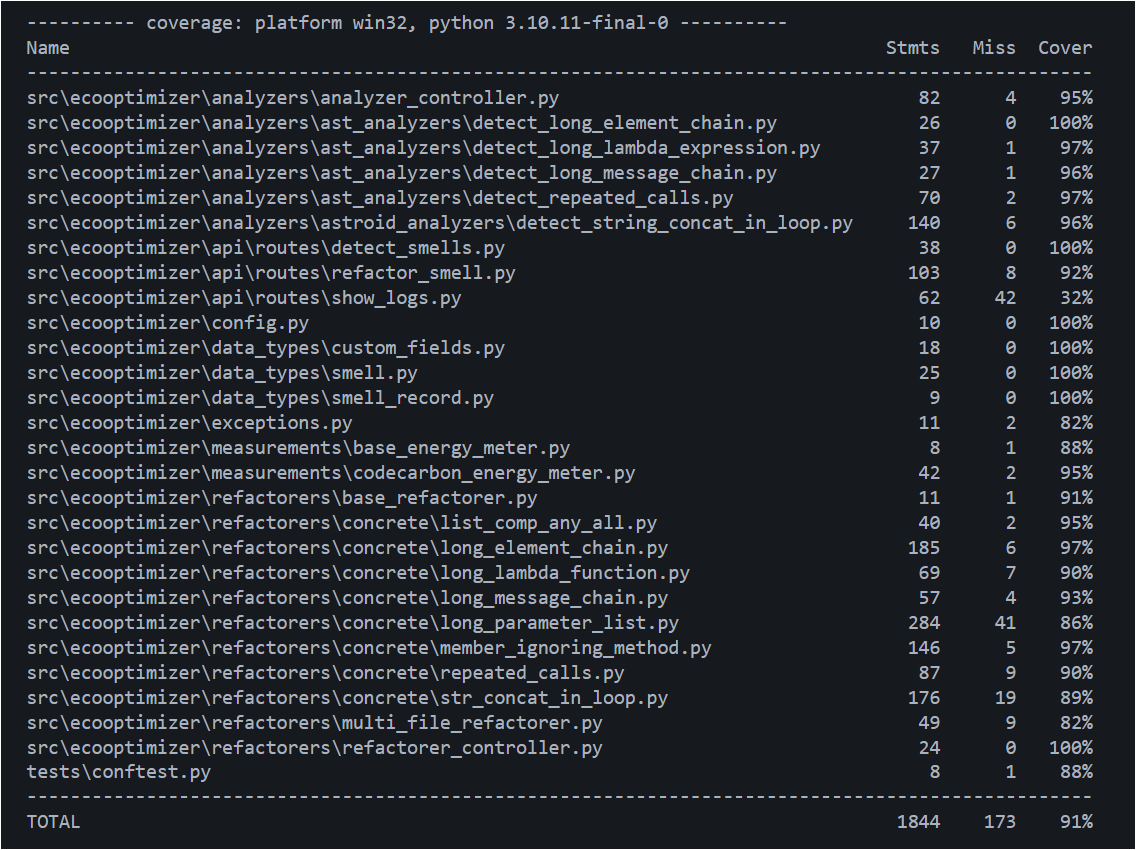
\includegraphics[width=0.7\textwidth]{../Images/python-coverage.png}
  \label{img:python-cov}
  \caption{Coverage Report of the Python Backend Library}
\end{figure}

\begin{figure}[H]
  \centering
  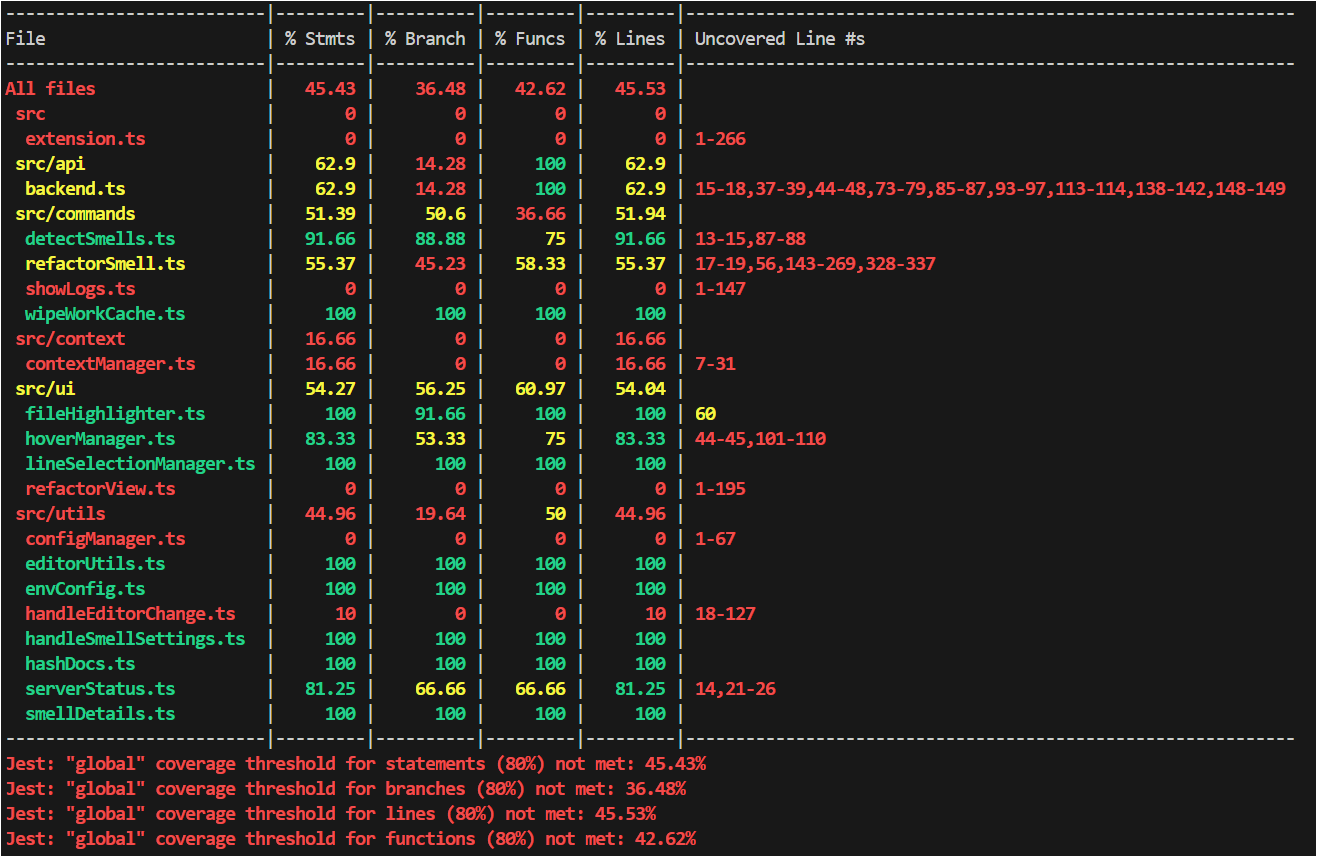
\includegraphics[width=0.7\textwidth]{../Images/vscode-coverage.png}
  \label{img:vscode-cov}
  \caption{Coverage Report of the VSCode Extension}
\end{figure}

\subsection{VSCode Extension}
The frontend codebase has an overall coverage of 45.43\% for statements, 36.48\% for branches, 42.62\% for functions, and 45.53\% for lines (\ref{img:vscode-cov}). These metrics fall below the global coverage thresholds of 80\% for the following reasons. The file \texttt{extension.ts}, which contains the core logic for the VSCode extension, has 0\% coverage as it is mainly made up of initialization commands with no real logic that can be tested. The file \texttt{refactorView.ts}, responsible for the refactoring view, also has 0\% coverage. This module is a UI component and will be tested for revision 1. Since \texttt{handleEditorChange.ts} is closely related to the UI component, its testing has also been put off.\\

The file \texttt{refactorSmell.ts} has moderate coverage (55.37\% statements, 45.23\% branches), with significant gaps in testing around lines 143–269 and 328–337 (Image 2). This is due to a feature that is not fully implemented and therefore not tested. Finally, \texttt{configManager.ts} has not been tested as yet due to evolving configuration options, but will be tested for revision 1.

\subsection{Python Backend}
The backend codebase has an overall coverage of 91\% (Image 1) and has been thoroughly tested as it contains the key features of project and the bulk of the logic. The exception is \texttt{show\_logs.py}, which handles the websocket endpoint for logging, due to the complex nature of this module testing has been omitted. Since its function is mainly to broadcast logs it is also relatively simple to verify its functionality manually\\


\bibliographystyle{plainnat}
\bibliography{../../refs/References}

\newpage
\section*{Appendix A -- Usability Testing Data} \label{appendix:usability}

\subsection*{Protocol}

\section*{Purpose}
The purpose of this usability test is to evaluate the ease of use, efficiency, and overall user experience of the VSCode extension for refactoring Python code to improve energy efficiency. The test will identify usability issues that may hinder adoption by software developers.

\section*{Objective}
Evaluate the usability of the extension’s \textbf{smell detection}, \textbf{refactoring process}, \textbf{customization settings}, and \textbf{refactoring view}.

\begin{itemize}
    \item Assess how easily developers can navigate the extension interface.
    \item Measure the efficiency of the workflow when applying or rejecting refactorings.
    \item Identify areas of confusion or frustration.
\end{itemize}

\section*{Methodology}
\subsection*{Test Type}
Moderated usability testing.

\subsection*{Participants}
\begin{itemize}
    \item \textbf{Target Users:} Python developers who use VSCode.
    \item \textbf{Number of Participants:} 5–7.
    \item \textbf{Recruitment Criteria:}
        \begin{itemize}
            \item Experience with Python development.
            \item Familiarity with VSCode.
            \item No prior experience with this extension.
        \end{itemize}
\end{itemize}

\subsection*{Testing Environment}
\begin{itemize}
    \item \textbf{Hardware:} Provided computer.
    \item \textbf{Software:}
        \begin{itemize}
            \item VSCode (latest stable release).
            \item The VSCode extension installed.
            \item Screen recording software (optional, for post-test analysis).
            \item A sample project with \textbf{predefined code snippets} containing various \textbf{code smells}.
        \end{itemize}
    \item \textbf{Network Requirements:} Stable internet connection for remote testing.
\end{itemize}

\subsection*{Test Moderator Role}
\begin{itemize}
    \item Introduce the test and explain objectives.
    \item Observe user interactions without providing assistance unless necessary.
    \item Take notes on usability issues, pain points, and confusion.
    \item Ask follow-up questions after each task.
    \item Encourage participants to \textbf{think aloud}.
\end{itemize}

\section*{Data Collection}
\subsection*{Metrics}
\begin{itemize}
    \item \textbf{Task Success Rate:} Percentage of users who complete tasks without assistance.
    \item \textbf{Error Rate:} Number of errors or missteps per task.
    \item \textbf{User Satisfaction:} Post-test rating on a scale of 1–5.
\end{itemize}

\subsection*{Qualitative Data}
\begin{itemize}
    \item Observations of confusion, hesitation, or frustration.
    \item Participant comments and feedback.
    \item Follow-up questions about expectations vs. actual experience.
    \item Pre-test survey.
    \item Post-test survey.
\end{itemize}

\section*{Analysis and Reporting}
\begin{itemize}
    \item Identify common pain points and recurring issues.
    \item Categorize usability issues by severity:
        \begin{itemize}
            \item \textbf{Critical:} Blocks users from completing tasks.
            \item \textbf{Major:} Causes significant frustration but has workarounds.
            \item \textbf{Minor:} Slight inconvenience, but doesn’t impact core functionality.
        \end{itemize}
    \item Provide recommendations for UI/UX improvements.
    \item Summarize key findings and next steps.
\end{itemize}

\section*{Next Steps}
\begin{itemize}
    \item Fix major usability issues before release.
    \item Conduct follow-up usability tests if significant changes are made.
    \item Gather further feedback from real users post-release.
\end{itemize}

\subsection*{Task List}

\section*{Mock Installation Documentation}
The extension can be installed to detect energy inefficiencies (smells) in your code and refactor them.

\subsection*{Commands}
Open the VSCode command palette (\texttt{CTRL+SHIFT+P}):

\begin{itemize}
    \item \textbf{Detect Smells:} \texttt{Eco: Detect Smells}
    \item \textbf{Refactor Smells:} \texttt{Eco: Refactor Smell} or \texttt{CTRL+SHIFT+R} (or to be discovered).
\end{itemize}

\section*{Tasks}
Report your observations \textbf{aloud}!

\subsection*{Task 1: Smell Detection}
\begin{enumerate}
    \item Open the \texttt{sample.py} file.
    \item Detect the smells in the file.
    \item What do you see?
\end{enumerate}

\subsection*{Task 2: Line Selection}
\begin{enumerate}
    \item In the same \texttt{sample.py} file, select one of the highlighted lines.
    \item What do you see?
    \item Select another line.
\end{enumerate}

\subsection*{Task 3: Hover}
\begin{enumerate}
    \item In the same file, hover over a highlighted line.
    \item What do you see?
\end{enumerate}

\subsection*{Task 4: Initiate Refactoring (Single)}
\begin{enumerate}
    \item In the same file, refactor any smell of your choice.
    \item What do you observe immediately after?
    \item Does a sidebar pop up after some time?
\end{enumerate}

\subsection*{Task 5: Refactor Smell (Sidebar)}
\begin{enumerate}
    \item What information do you see in the sidebar?
    \item Do you understand the information communicated?
    \item Do you see what was changed in the file?
    \item Try rejecting a smell. Did the file change?
    \item Repeat Tasks 1, 4, and 5, but reject a smell. Did the file stay the same?
\end{enumerate}

\subsection*{Task 6: Refactor Multi-File Smell}
\begin{enumerate}
    \item Open the \texttt{main.py} file.
    \item Detect the smells in the file.
    \item Refactor any smell of your choice.
    \item Do you see anything different in the sidebar?
    \item Try clicking on the new addition to the sidebar. Notice anything?
    \item Try accepting the refactoring. Did both files change?
\end{enumerate}

\subsection*{Task 7: Change Smell Settings}
\begin{enumerate}
    \item Open the \texttt{sample.py} file.
    \item Detect the smells in the file.
    \item Take note of the smells detected.
    \item Open the settings page (\texttt{CTRL+,}).
    \item Navigate to the \textbf{Extensions} drop-down and select \textbf{Eco Optimizer}.
    \item Unselect one of the smells you noticed earlier.
    \item Navigate back to the \texttt{sample.py} file.
    \item Detect the smells again. Is the smell you unselected still there?
\end{enumerate}

\subsection*{Participant Data}
The following links point to the data collected from each participant:\\

{\noindent
\href{run:./../Extras/UsabilityTesting/test_data/participant1-data.csv}{Participant 1} \\[2mm]
\href{run:./../Extras/UsabilityTesting/test_data/participant2-data.csv}{Participant 2} \\[2mm]
\href{run:./../Extras/UsabilityTesting/test_data/participant3-data.csv}{Participant 3} \\[2mm]
\href{run:./../Extras/UsabilityTesting/test_data/participant4-data.csv}{Participant 4} \\[2mm]
\href{run:./../Extras/UsabilityTesting/test_data/participant5-data.csv}{Participant 5}
}

\subsection*{Pre-Test Survey Data}
The following link points to a CSV file containing the pre-survey data:\\

\noindent
\href{run:./../Extras/UsabilityTesting/surveys/pre-test-survey-data.csv}{Click here to access the survey results CSV file}.

\subsection*{Post-Test Survey Data}
The following link points to a CSV file containing the post-survey data:\\

\noindent
\href{run:./../Extras/UsabilityTesting/surveys/post-test-survey-data.csv}{Click here to access the survey results CSV file}.

\newpage{}
\section*{Appendix --- Reflection}

The information in this section will be used to evaluate the team members on the
graduate attribute of Reflection.

\input{../Reflection.tex}

\begin{enumerate}
  \item What went well while writing this deliverable? 
  \item What pain points did you experience during this deliverable, and how
    did you resolve them?
  \item Which parts of this document stemmed from speaking to your client(s) or
  a proxy (e.g. your peers)? Which ones were not, and why?
  \item In what ways was the Verification and Validation (VnV) Plan different
  from the activities that were actually conducted for VnV?  If there were
  differences, what changes required the modification in the plan?  Why did
  these changes occur?  Would you be able to anticipate these changes in future
  projects?  If there weren't any differences, how was your team able to clearly
  predict a feasible amount of effort and the right tasks needed to build the
  evidence that demonstrates the required quality?  (It is expected that most
  teams will have had to deviate from their original VnV Plan.)
\end{enumerate}

\end{document}